\documentclass[3p,final,twocolumn]{elsarticle}

\usepackage{lineno,hyperref}

\usepackage{graphicx}% Include figure files
\usepackage{dcolumn}% Align table columns on decimal point
\usepackage{amsmath}
\usepackage{amssymb}
\usepackage{epstopdf}
\usepackage{multirow}
\usepackage{color}
%\usepackage{longtable}
\usepackage{braket}
%\usepackage{hepparticles} % particle names
%\usepackage{hepnames} % shortcuts for lots of particle names
\usepackage[alsoload=hep]{siunitx}
\sisetup{ per-mode=symbol}

\usepackage{subcaption}
%\captionsetup[subfigure]{labelformat = parens, labelsep = space, font = small}


\graphicspath{{figures/}}

\modulolinenumbers[5]

\journal{}
\bibliographystyle{elsarticle-num}


%%%%%%%%%%%%%%%%%%%%%%%%%%%%%%%%%%%%%%%%%%%% 
\newcommand*{\MIT }{Massachusetts Institute of Technology, Cambridge, Massachusetts 02139, USA}
\newcommand*{\ODU}{Old Dominion University, Norfolk, Virginia 23529}
\newcommand*{\JLAB}{Thomas Jefferson National Accelerator Facility, Newport News, Virginia 23606}
\newcommand*{\TAU }{School of Physics and Astronomy, Tel Aviv University, Tel Aviv 69978, Israel}
\newcommand*{\Penn}{Pennsylvania State University, University Park, PA, 16802}
\newcommand*{\NRC}{Nuclear Research Center Negev, Be'er Sheva 84190, Israel}


\begin{document}


%%%%%%%%%%%%%%%%%%%%%%%%%%%%%%%%%%%%%%%%%%%%%%%%%%%%%%%%%%%%%%%%%%%%%%%%%%%%%%%%%%%%%%%%%%%%%%%%%%%
\begin{frontmatter}

\title{The CLAS12 Backward Angle Neutron Detector (BAND) }

%% Group authors per affiliation:
\author{E.P.~Segarra, F.~Hauenstein, A.~Schmidt, R.~Cruz-Torres, \\O.~Hen, A.~Denniston, T.~Kutz, J.~Pybus, A.~Hrnjic\\A.~Nambrath, A.~Beck, S.~May-Tal Beck\corref{mycorrespondingauthor}}
\address{\MIT}
\author{C.~Fogler, L.B.~Weinstein, T.~Hartlove}
\address{\ODU}
\author{I.~Vega, M.~Mu\~nos, H.~Hakobyan, W.~Brooks}
\address{UTFSM}
\author{E.~Piasetzky, E.~Cohen, M.~Duer}
\address{\TAU}
\author{K.~Pryce}
\address{Orsay}
\author{P.~Eugenio}
\address{FSU}
\author{I.~Korover}
\address{\NRC}
\author{P.~Correa}
\address{}

%%%%%%%%%%%%%%%%%%%%%%%%%%%%%%%%%%%%%%%%%%%%%%%%%%%%%%%%%%%%%%%%%%%%%%%%%%%%%%%%%%%%%%%%%%%%%%%%%%%
\author[]{}
\ead[]{}

\begin{abstract}
The Backward Angle Neutron Detector (BAND) of CLAS12 is discussed. The detector is positioned $3$ \si{\meter} upstream of the target and is used to 
detect neutrons emitted at backward angles of $155$\si{\degree} to $175$\si{\degree} and momenta between $0.25$ and $0.6$ \si{\GeV/\clight}. It consists of $18$ rows and $5$ layers of $7.2$ \si{\centi\meter} 
by $7.2$ \si{\centi\meter} scintillator bars with PMT readout on both ends to measure the neutron time-of-flight from the target and the 
energy deposition in the scintillator layers. The face of the detectors includes a $2.5$ \si{\centi\meter} thick lead wall followed by a $1$ \si{\centi\meter} veto layer to suppress gammas and reject charged particles. The detector achieves a  detection efficiency of 
$35$\% at xx \si{\MeV/\clight} with a momentum reconstruction resolution of $<1.5$\%.
\end{abstract}

\begin{keyword}
CLAS12; Time of flight; Plastic scintillator; Fast neutrons
\end{keyword}
\end{frontmatter}

%%%%%%%%%%%%%%%%%%%%%%%%%%%%%%%%%%%%%%%%%%%%%%%%%%%%%%%%%%%%%%%%%%%%%%%%%%%%%%%%%%%%%%%%%%%%%%%%%%%
\linenumbers

\section{Introduction}


The CLAS12 (Cebaf Large Angle Spectrometer) \cite{Burkert:2020akg} at HallB of the Thomas Jefferson National Acclerator facility (JLab) is a multi-purpose spectrometer used to detect charged and neutral particles. It covers angles from xx to xx and momenta from xx to xx for the different particles. 
Tagged deep inelastic scattering studies in $ed$ reactions require the detection of recoil neutrons with momenta above \SI{250}{\mega\eVperc} at backward angles. Therefore, a new detector has been build to detect these neutrons, the Backward Angle Neutron Detector (BAND). A model representation of BAND and CLAS12 is shown in Fig.~\ref{fig:clas12band} to highlight the overall layout and scale in HallB. BAND was installed in January 2019 and has been taken data in coincidence with CLAS12.

\begin{figure}[t!]
	\centering
	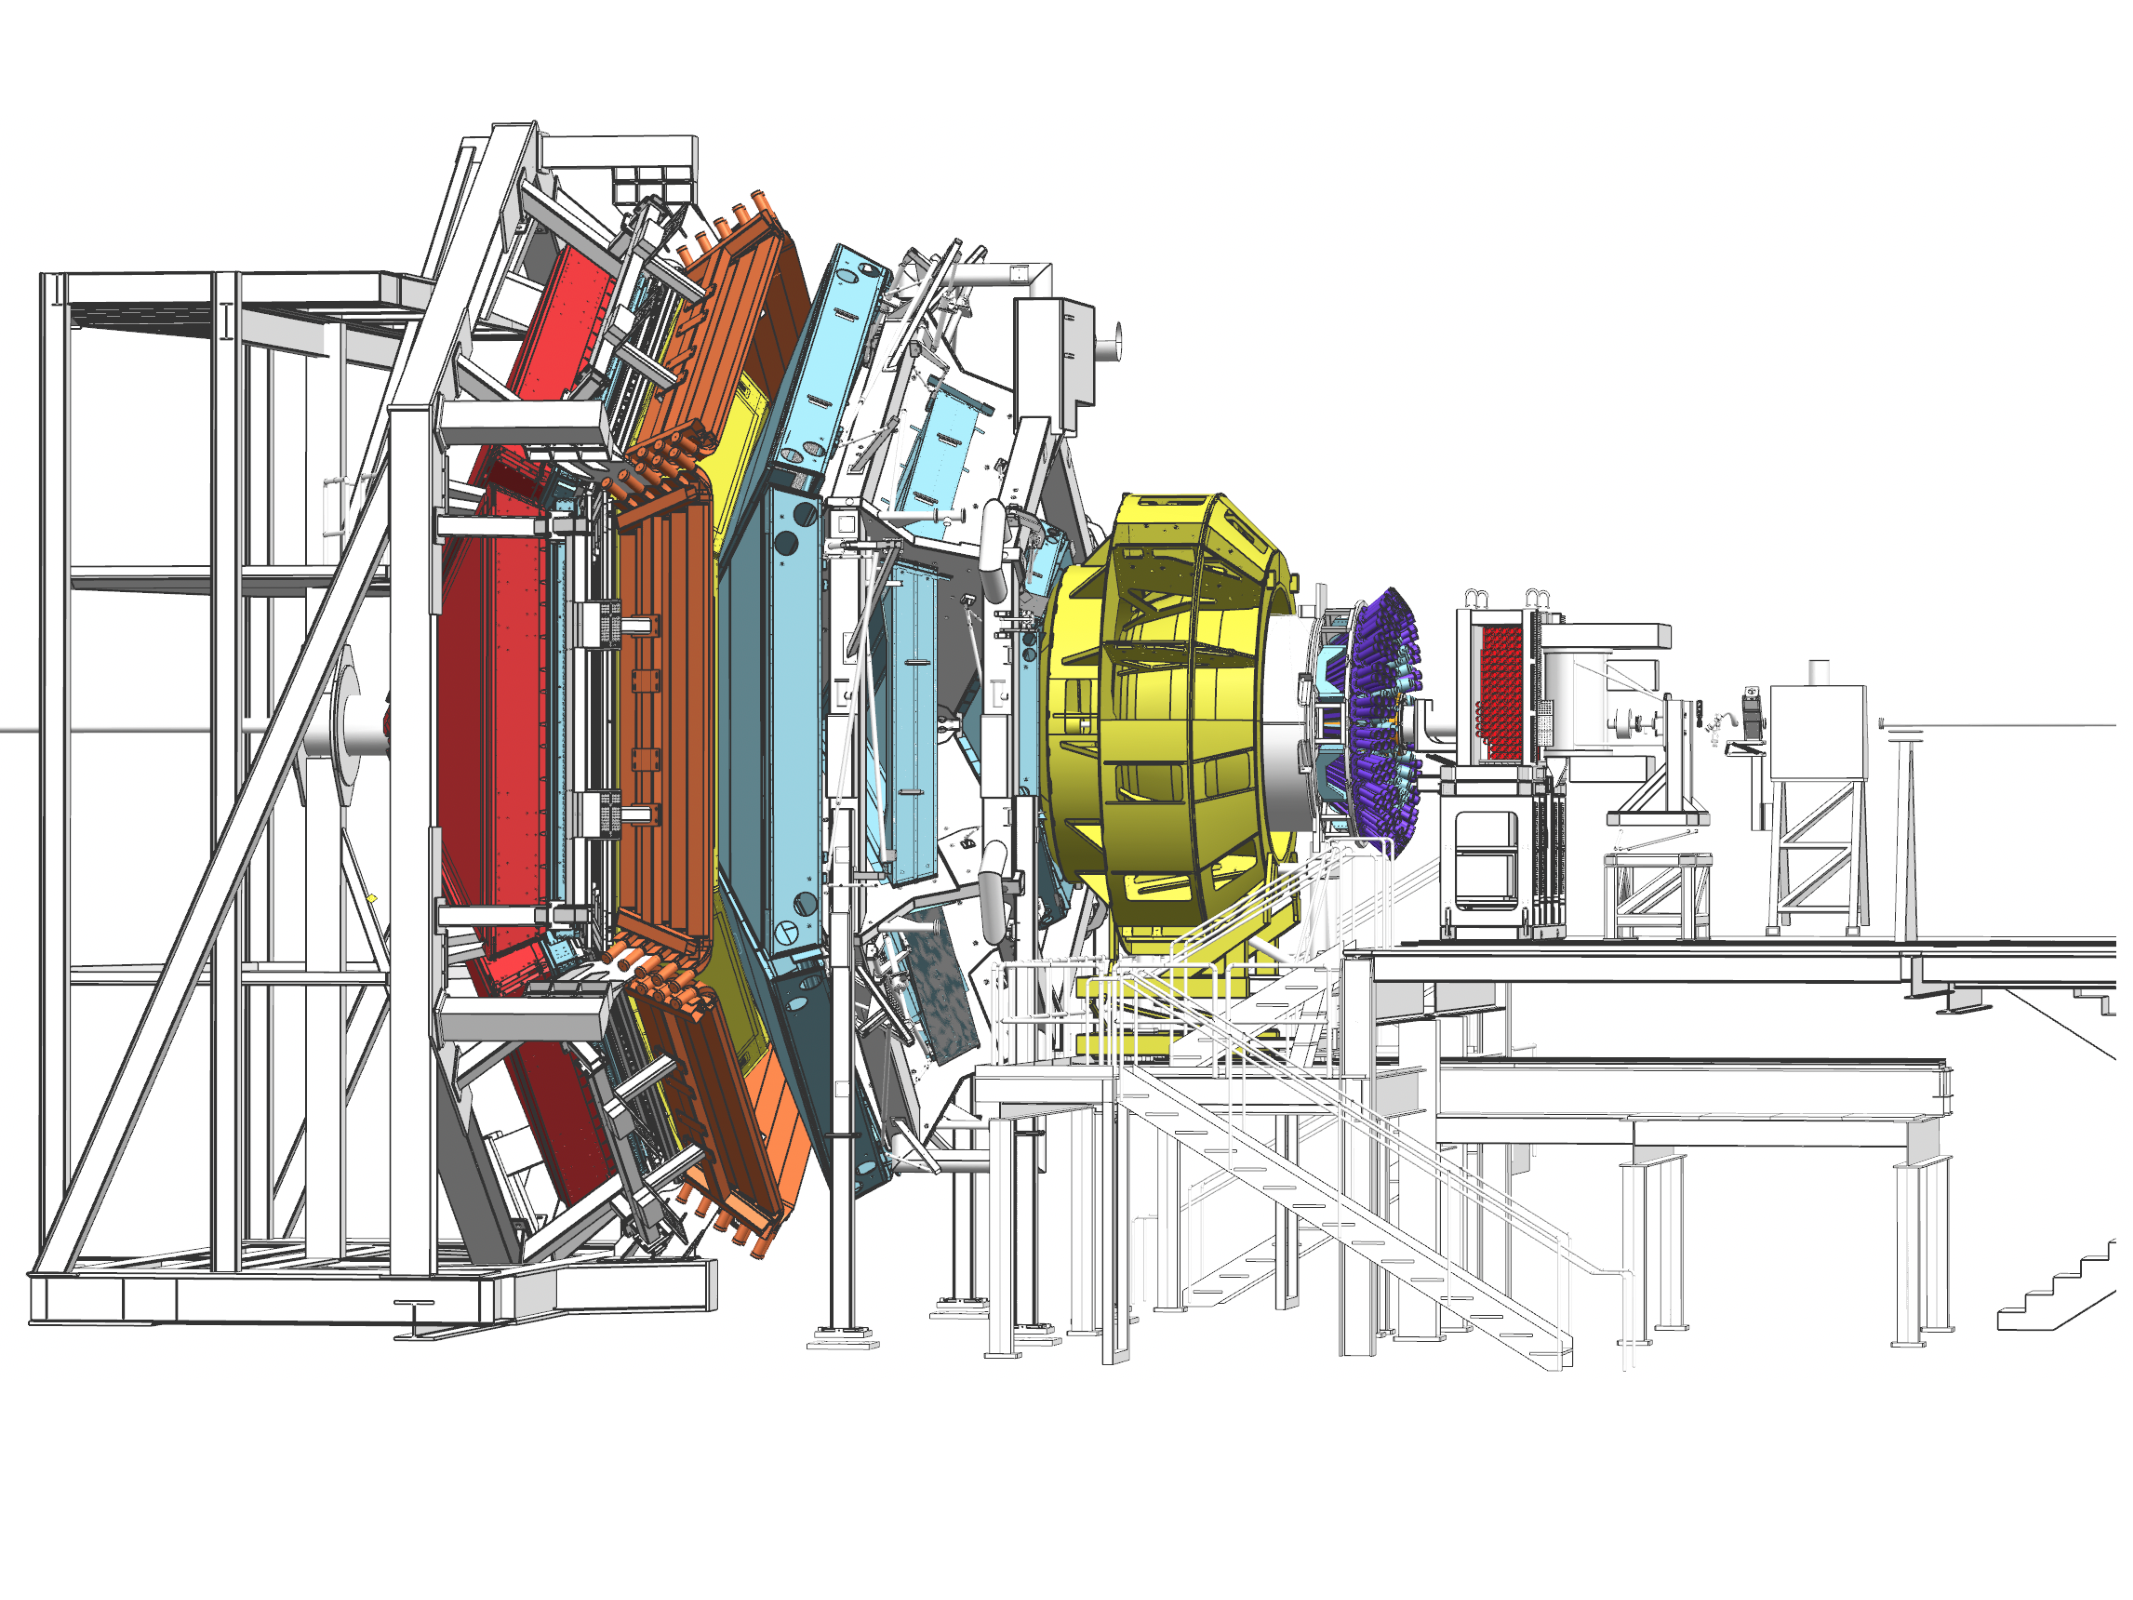
\includegraphics[width=0.48\textwidth]{BandInClas.pdf}
		\caption{Model representation of CLAS12 and BAND in HallB at Jefferson Lab. The electron beam is incident from the right side. BAND is marked in red. The overall detector system is roughly 20 \si{\meter} in scale along the beam axis. }
		\label{fig:clas12band}
\end{figure}

This newly build detector is designed to measure neutrons with momenta of $0.25 - 0.6$ \si{\GeV/\clight} with a detection efficiency of $35$\%  and angular coverage of $155$\si{\degree} to $175$\si{\degree}. It is based on scintillator bars with PMT readout. 

In this paper, we first review the general design of BAND and its requirements in terms of time resolution  and geometry. We then discuss the selection of the detector components,
comparative test bench measurements of different scintillators, PMTs and magnetic shields. In the following chapter, we present the performance of the detector after its installation in JLab's HallB. A detailed overview of the calibrations is given using mainly data from cosmic rays and a laser calibration system \cite{band-laser}. Finally, we present the measured time-of-flight (TOF) resolutions and neutron-photon separation from  data obtained with a $10.6$ \si{\GeV} electron beam impinding on a deuterium target.


%%%%%%%%%%%%%%%%%%%%%%%%%%%%%%%%%%%%%%%%%%%%%%%%%%%%%%%%%%%%%%%%%%%%%%%%%%%%%%%%%%%%%%%%%%%%%%%%%%%

\section{Design of the backward angle neutron detector}
To achieve the physics channels of interest with neutrons in the BAND \cite{band-proposal}, time-of-flight (ToF) resolutions below $300$ \si{\pico\second} are required for the scintillant detector with the average path length of about $3$ \si{\meter} {\color{red} shall we add more details here about why these parameters)}. Neutral-particle identification is established by vetoing on a thin $1$ \si{\centi\meter} veto layer for charged-particle identification between the target and the first active layer of BAND. Neutron-photon discrimination is achieved with ToF separation given the design 
timing resolutions. Furthermore, off-time random neutron contamination can be controlled with signal energy deposit. {\color{red} Any need to mention 
the raw rates that we need to handle in CLAS12?} .

%%ADD MORE WHAT IS SHOWN NEXT
%% ALSO TABLES FOR GEMOETRY< PMTS ADN SCINTILLATOR IN THIS CHAPTER. PART OF IT IN GEOMETRY
%%ALSO LIGHTGUIDES!!
%%GEMOETRY CONSTRAINTS: LENGTH BY SIZE, CROSS SECTION BY COSTS
\subsection{Geometry}

\begin{figure}[ht]
	\centering
		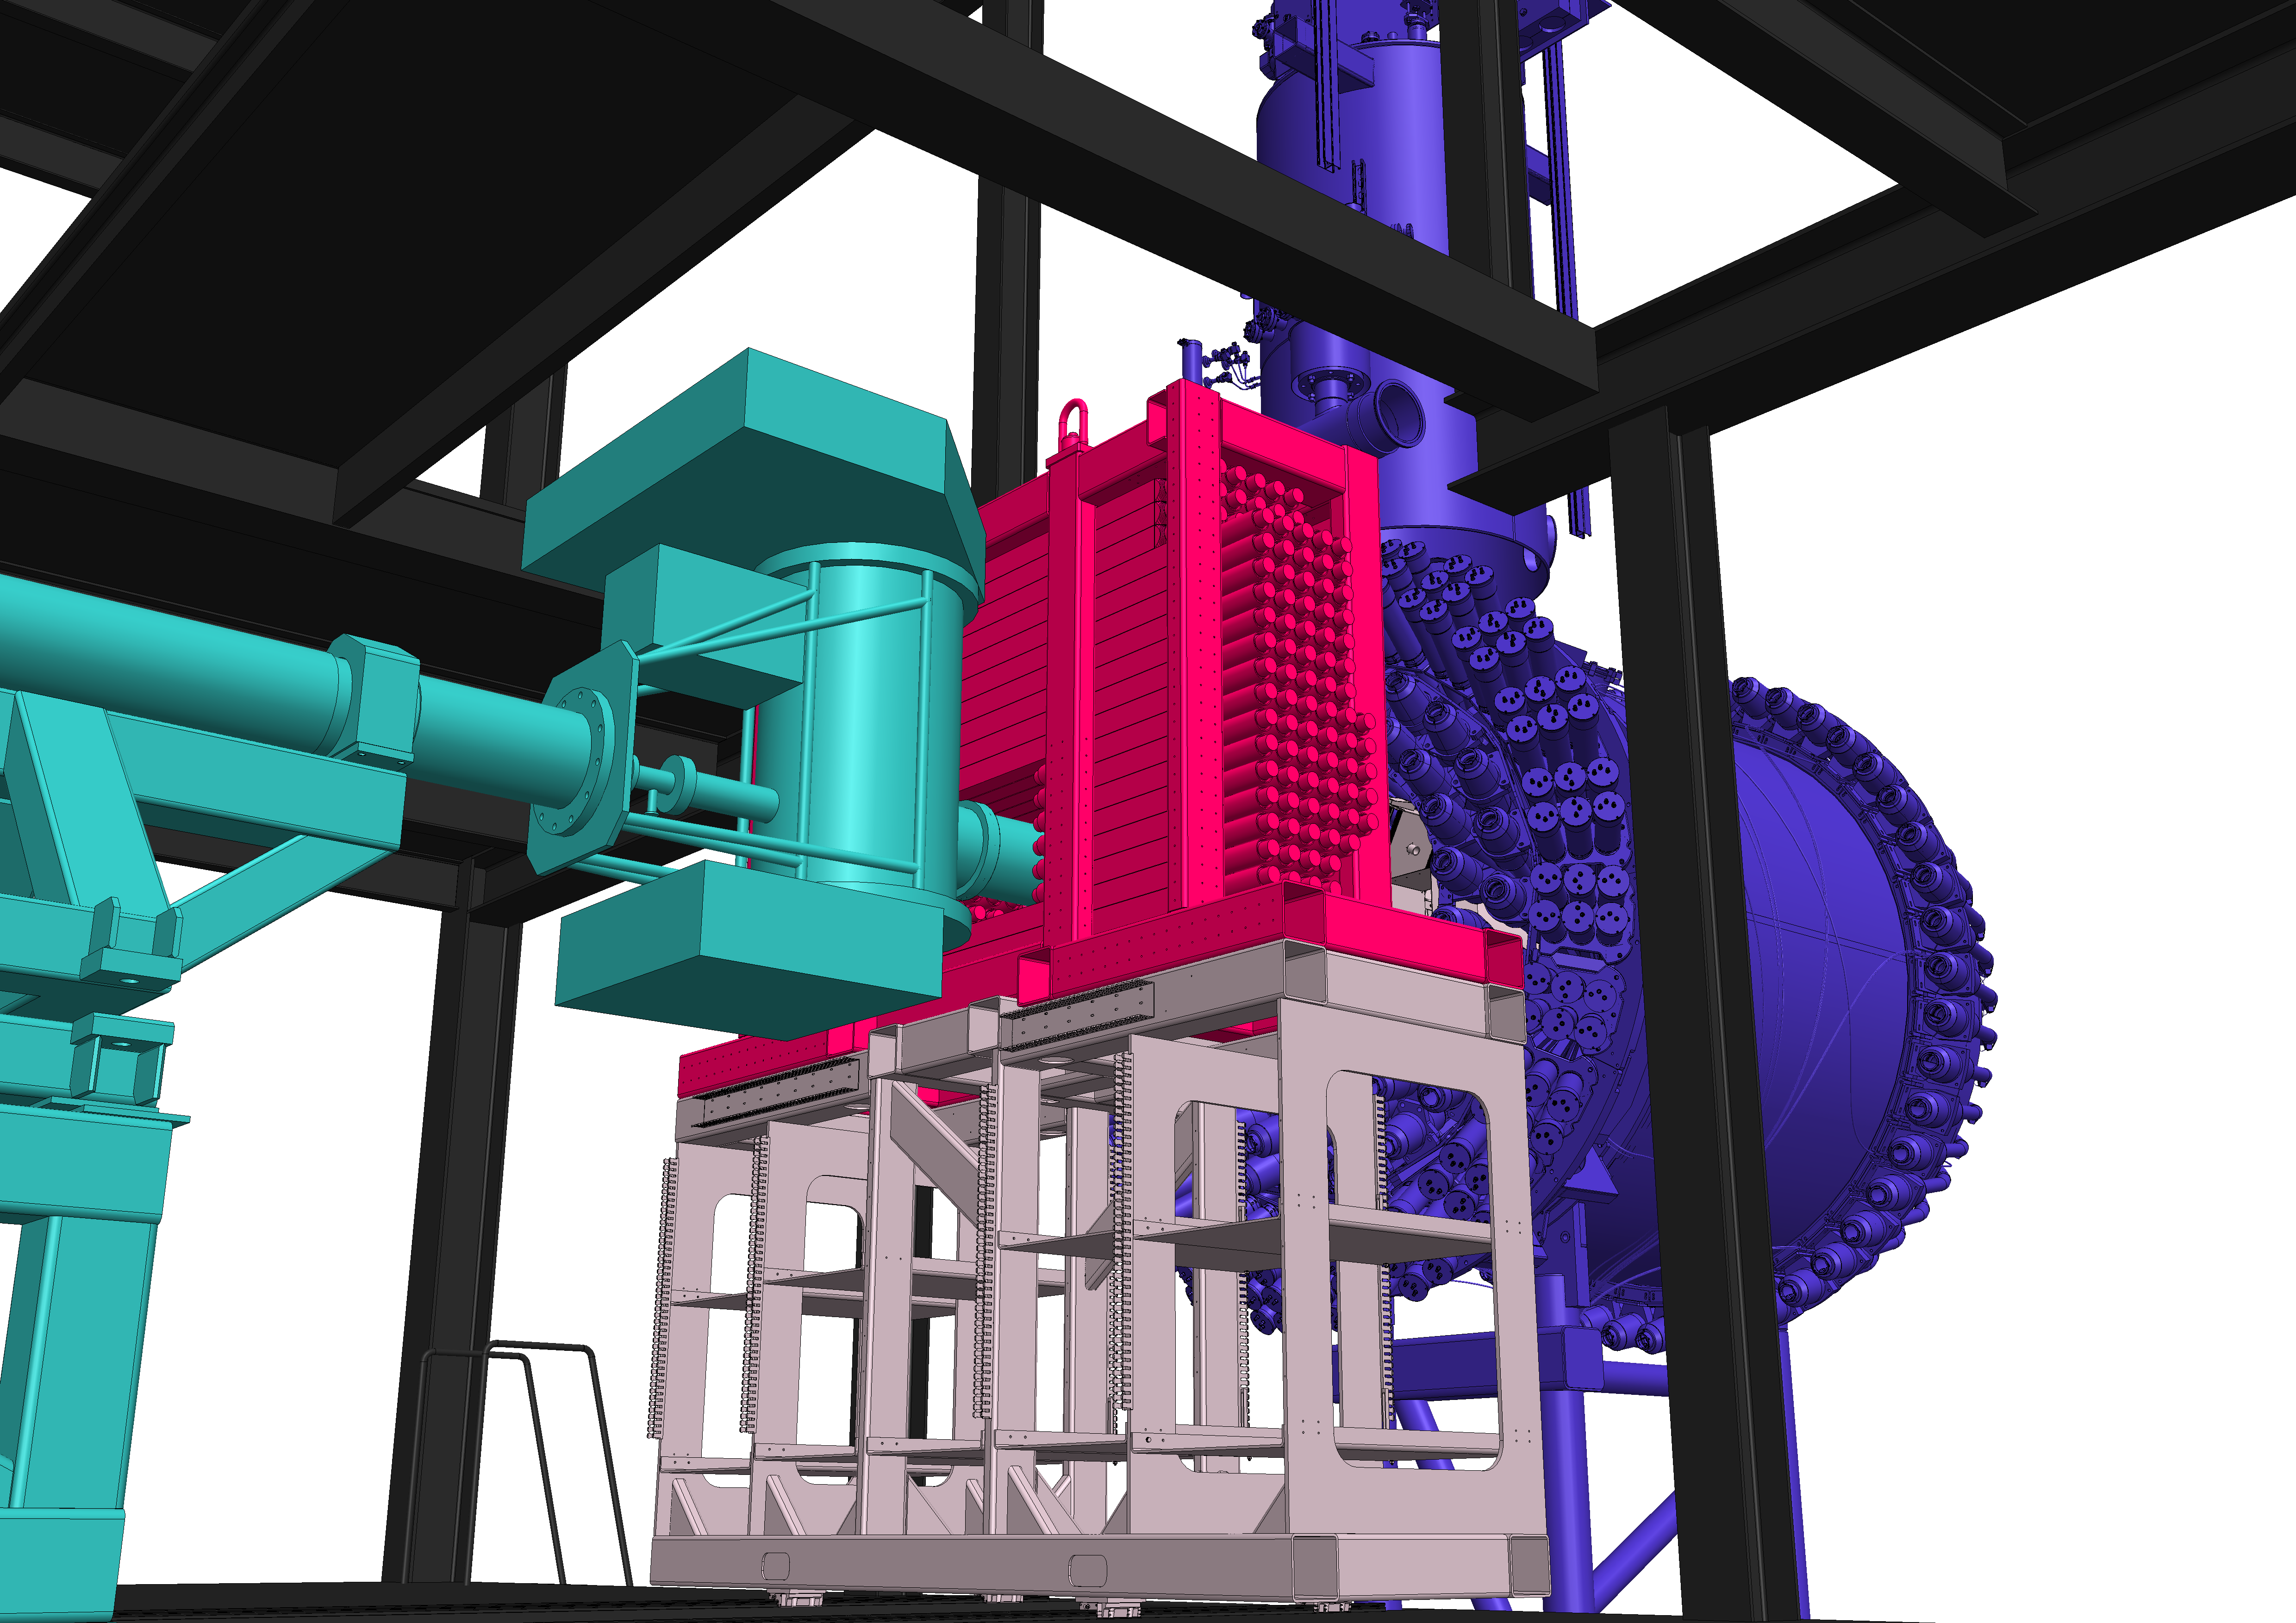
\includegraphics[width=0.48\textwidth]{FULL_CONTEXT_STUDIE_3.png}
		\caption{BAND and its close surroundings: the target is shown in cyan,  BAND in red and the central detector region of CLAS12 in blue. }
		\label{fig:bandtarget}
\end{figure}


\begin{figure}[ht]
	\centering
	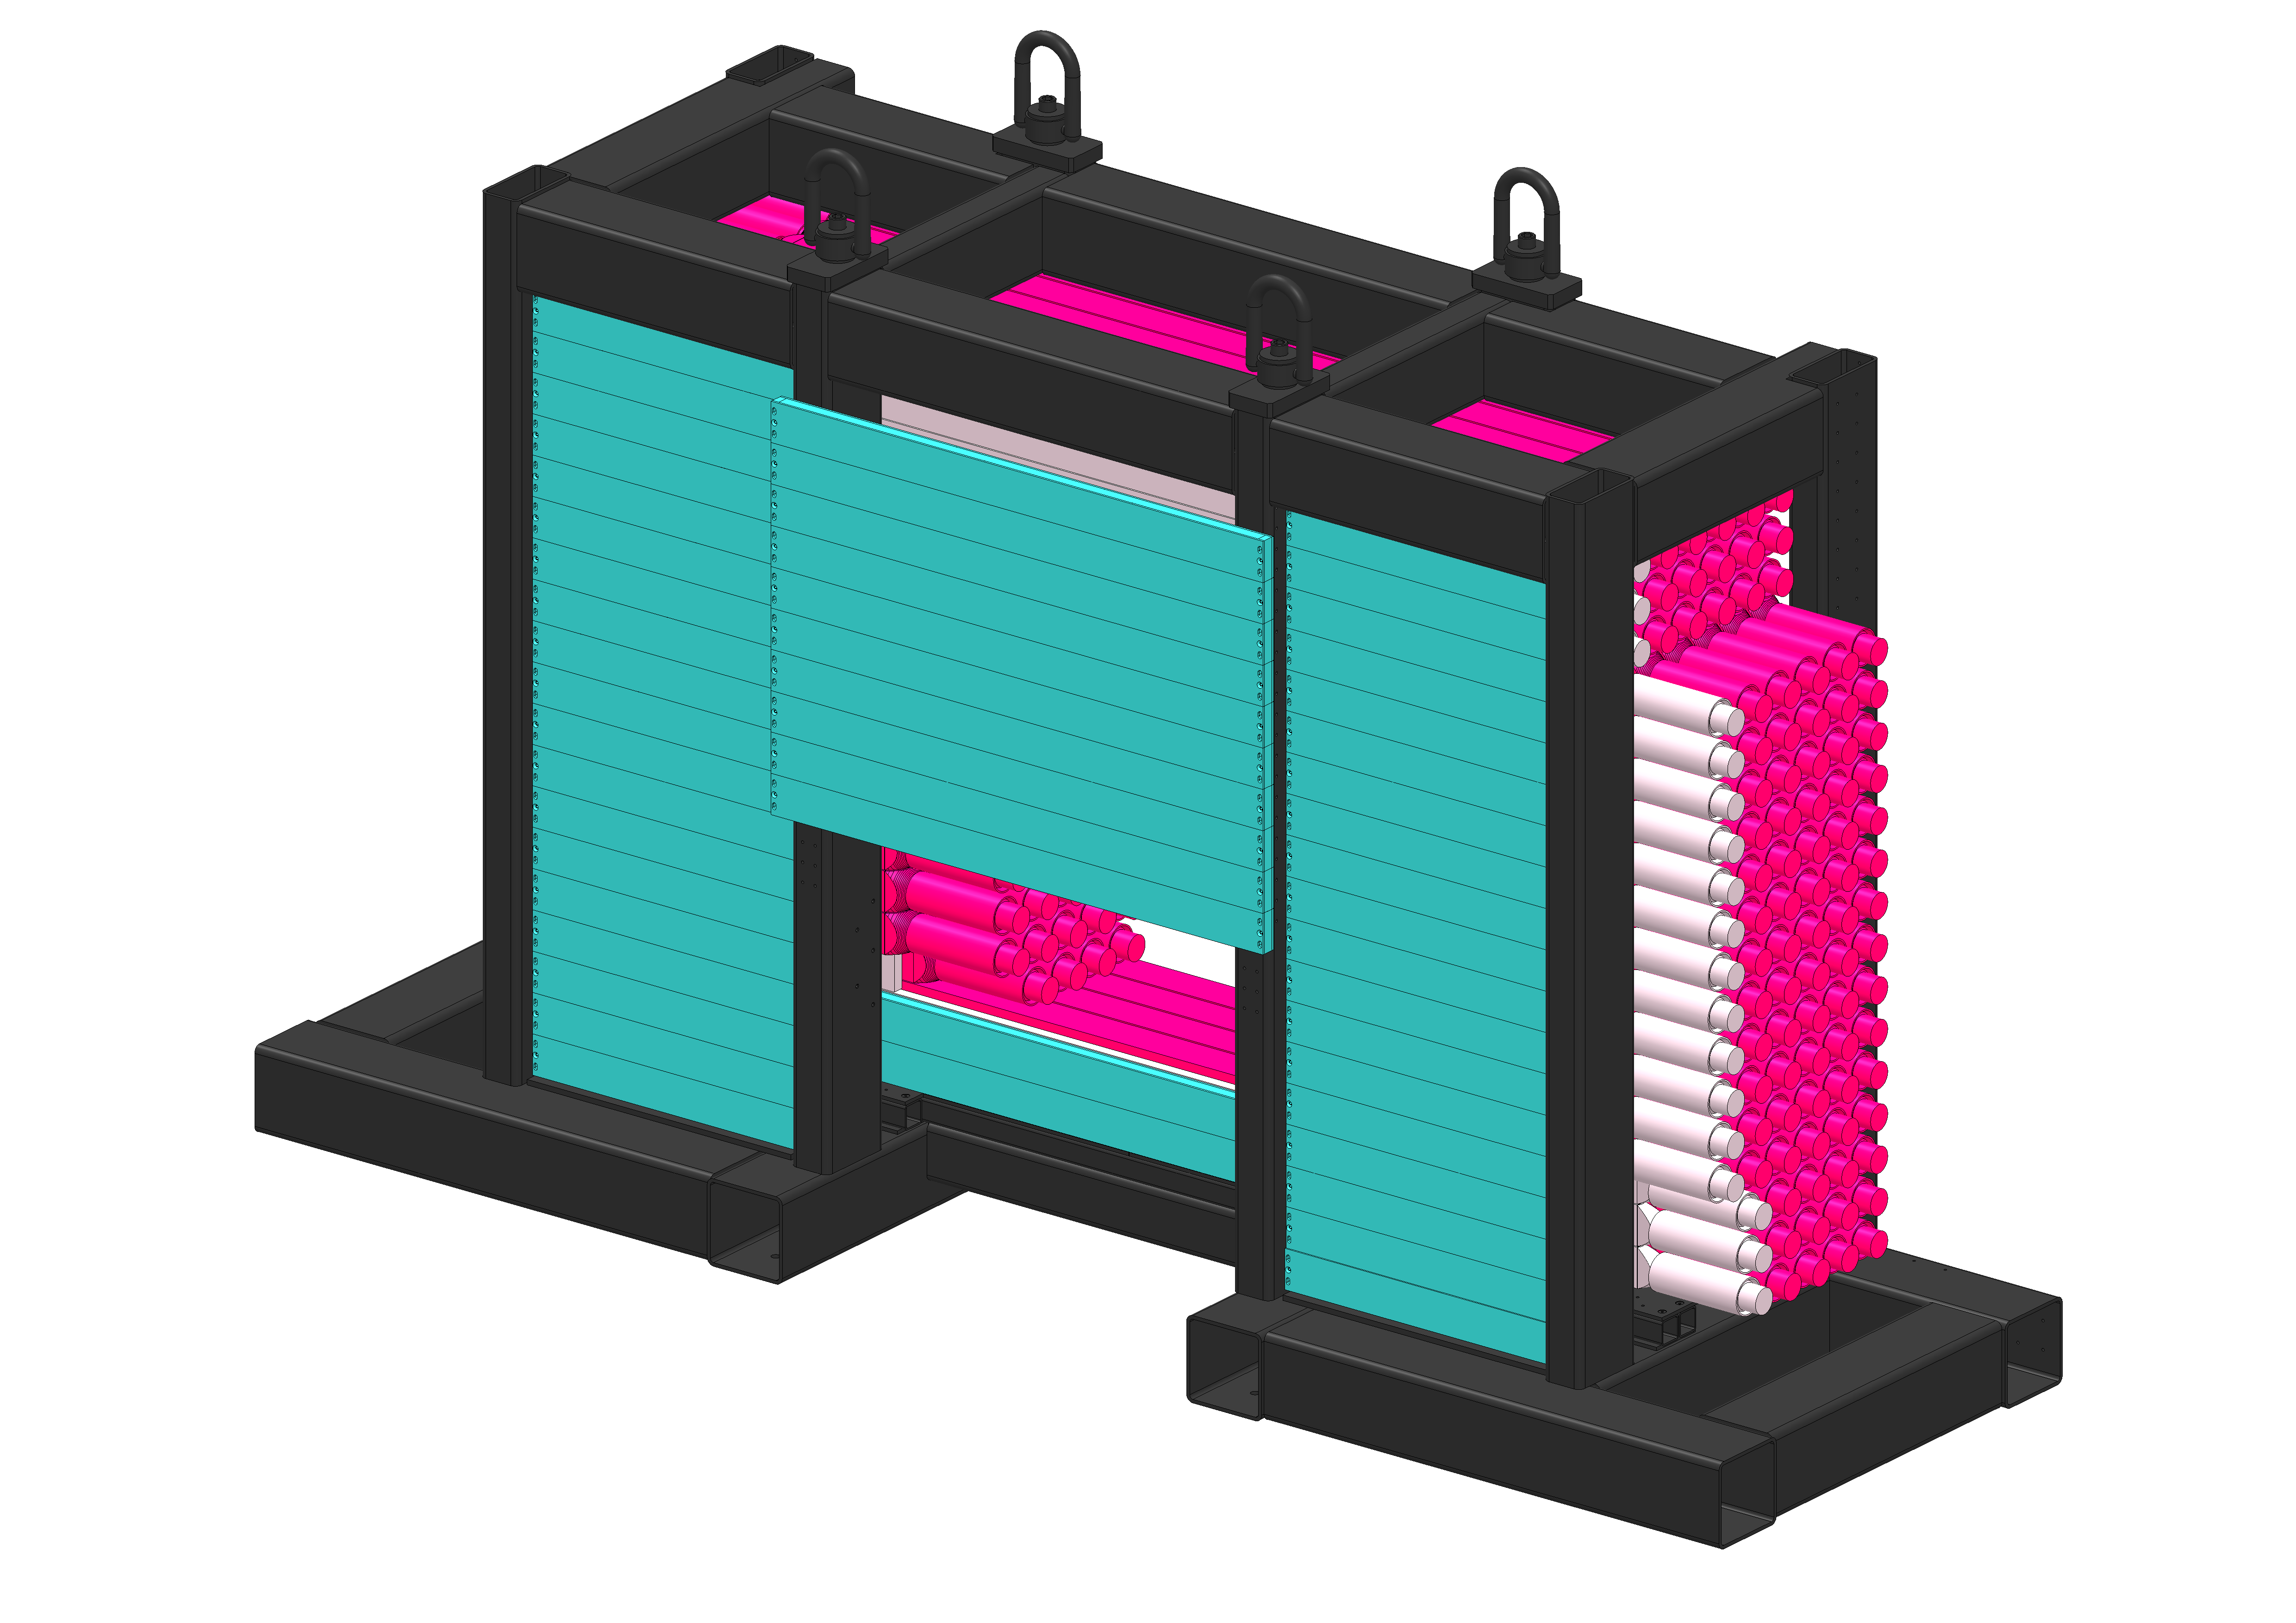
\includegraphics[width=0.48\textwidth]{BAND_1-2.png}
		\caption{BAND and its frame. The cyan color indicates the lead shield wall installed at the downstream side of BAND.}
		\label{fig:band}
\end{figure}


\begin{table*}[t]
\caption{{\color{red} THIS TABLE NEEDS AN UPDATE> IT IS JUST A TEMPORARY PLACEHOLDER WITH FTOF VALUES}Parameters for the scintillators, PMTs, and counters for the different BAND sectors and layers.}
\begin{center}
\begin{tabular} {c|l} \hline
~~Parameter~~ &~~~~~~~~~~~~~~~~~~~~~~ Design Value ~~~~~~~~~~\\ \hline
\multicolumn{2}{c} {Panel-1a (23 counters per sector)} \\
Angular Coverage      & $\theta = 5^\circ \to 35^\circ$, $\phi: 50\% {\rm ~at~} 5^\circ \to 85\% {\rm ~at~} 
35^\circ$ \\
Counter Dimensions   & $L = 32.3$~cm $\to$ 376.1~cm, $w \times h$ = 15~cm $\times$ 5~cm   \\
Scintillation Material & BC-408   \\
PMTs                         & EMI 9954A, Philips XP2262 \\
Counter Time Resolution     & 90~ps $\to$ 180~ps   \\ \hline
\multicolumn{2}{c} {Panel-1b (62 counters per sector)} \\
Angular Coverage      & $\theta = 5^\circ \to 35^\circ$, $\phi: 50\% {\rm ~at~} 5^\circ \to 85\% {\rm ~at~} 
35^\circ$ \\
Counter Dimensions   & $L = 17.3$~cm $\to$ 407.9~cm, $w \times h$ = 6~cm $\times$ 6~cm   \\
Scintillation Material & BC-404 (\#1 $\to$ \#31), BC-408 (\#32 $\to$ \#62)  \\
PMTs                         & Hamamatsu R9779 \\
Counter Time Resolution     & 60~ps $\to$ 110~ps   \\ \hline
\multicolumn{2}{c} {Panel-2 (5 counters per sector)} \\
Angular Coverage      & $\theta = 35^\circ \to 45^\circ$, $\phi: 85\% {\rm ~at~} 35^\circ \to 95\% {\rm ~at~} 
45^\circ$ \\
Counter Dimensions   & $L = 371.3$~cm $\to$ 426.1~cm, $w \times h$ = 22~cm $\times$ 5~cm   \\
Scintillation Material & BC-408   \\
PMTs                         & Photonis XP4312B, EMI 4312KB \\
Counter Time Resolution     & 170~ps $\to$ 180~ps   \\ \hline
\end{tabular}
\label{spec-table}
\end{center}
\end{table*}
%%%%%%%%%%%%%%%%%%%%%%%%%%%%%%%%%%%%%%%%%%%%%%%%%%%%%%%%%


The geometry of the BAND was constrained by the physics of interest (i.e. backward-going neutrons) [ADD REF] and the available space in the hall. To
maximize the fiducial volume inside of hall constraints, a design of rectangular scintillant bars that are layered perpendicular to the beam direction ($z$); see Fig.~\ref{fig:design}.
The cross section of each scintillator bar determines our position granularity in $y,z$ (vertical and longitudinal direction), and was chosen such that it yields comparable uncertainty to $x$ (horizontal direction) given the bar 
time resolutions. With a design ToF resolution below $300$ \si{\pico\second}, $7.2$ \si{\centi\meter} by $7.2$ \si{\centi\meter} scintillator bars were chosen to optimize
fiducial volume, granularity, and cost.
\begin{figure*}[h]
	\centering
		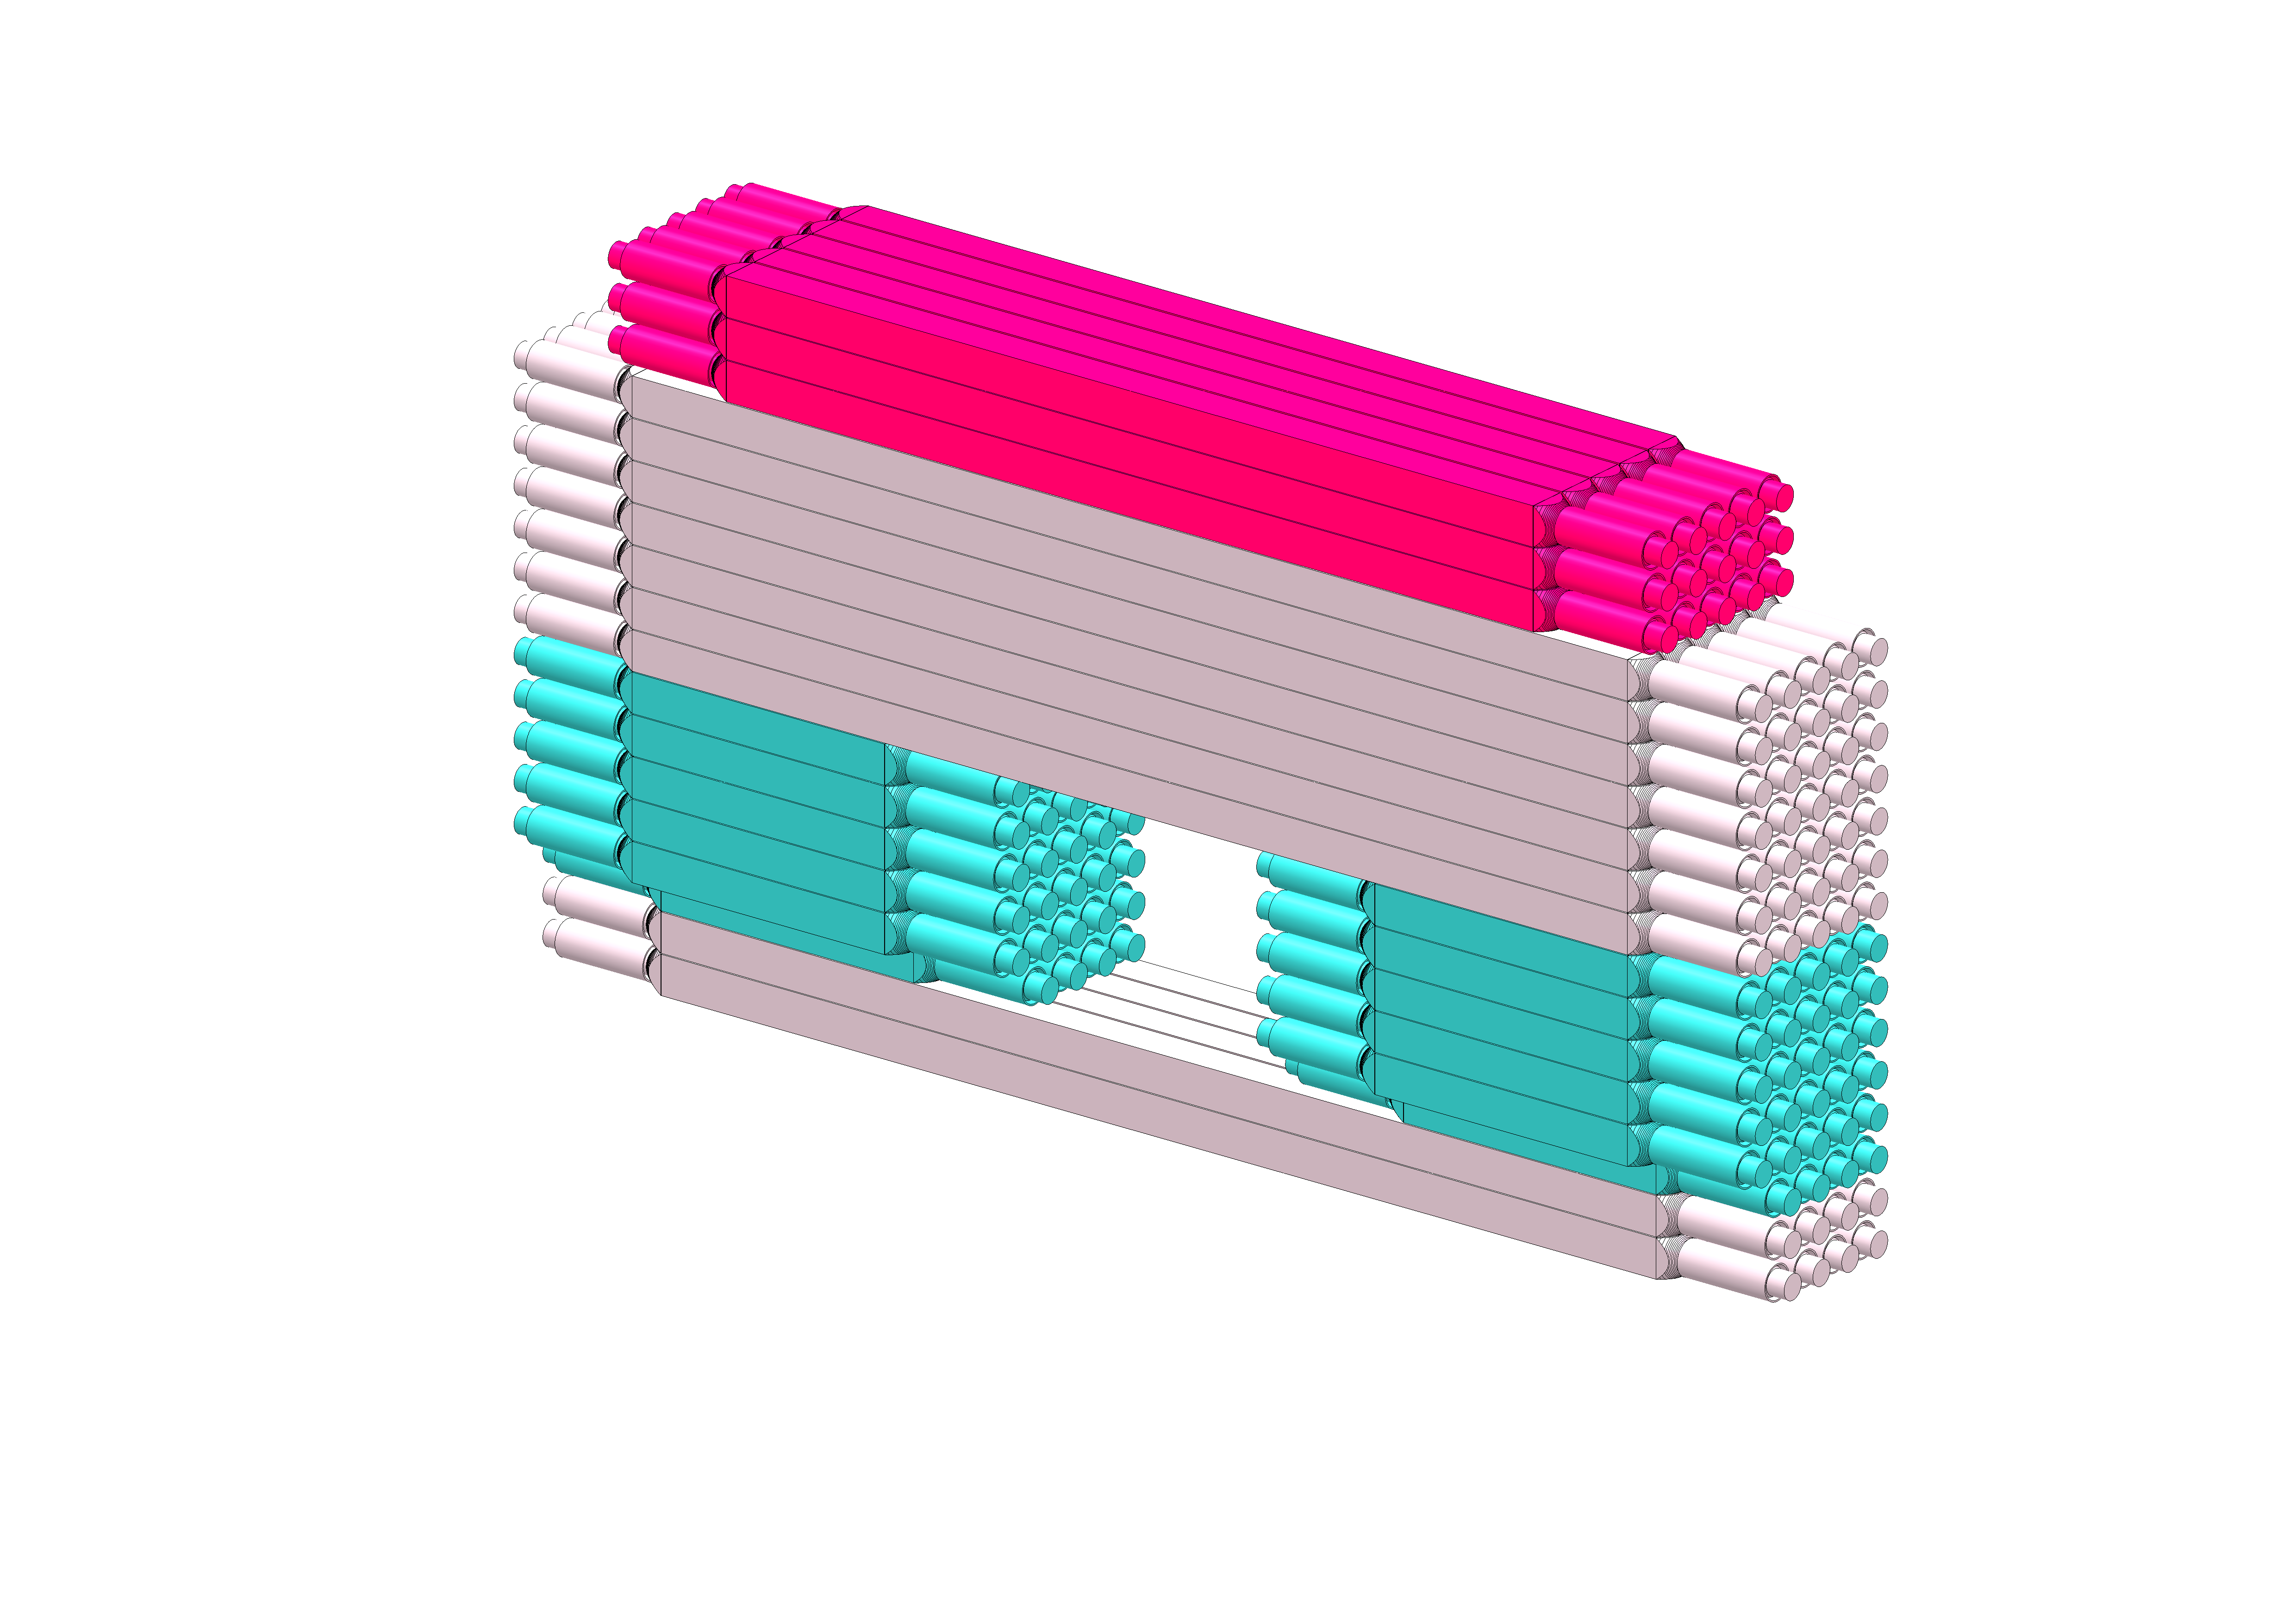
\includegraphics[width=0.48\textwidth]{MAIN_DETECTOR_COLORED_2.png}
		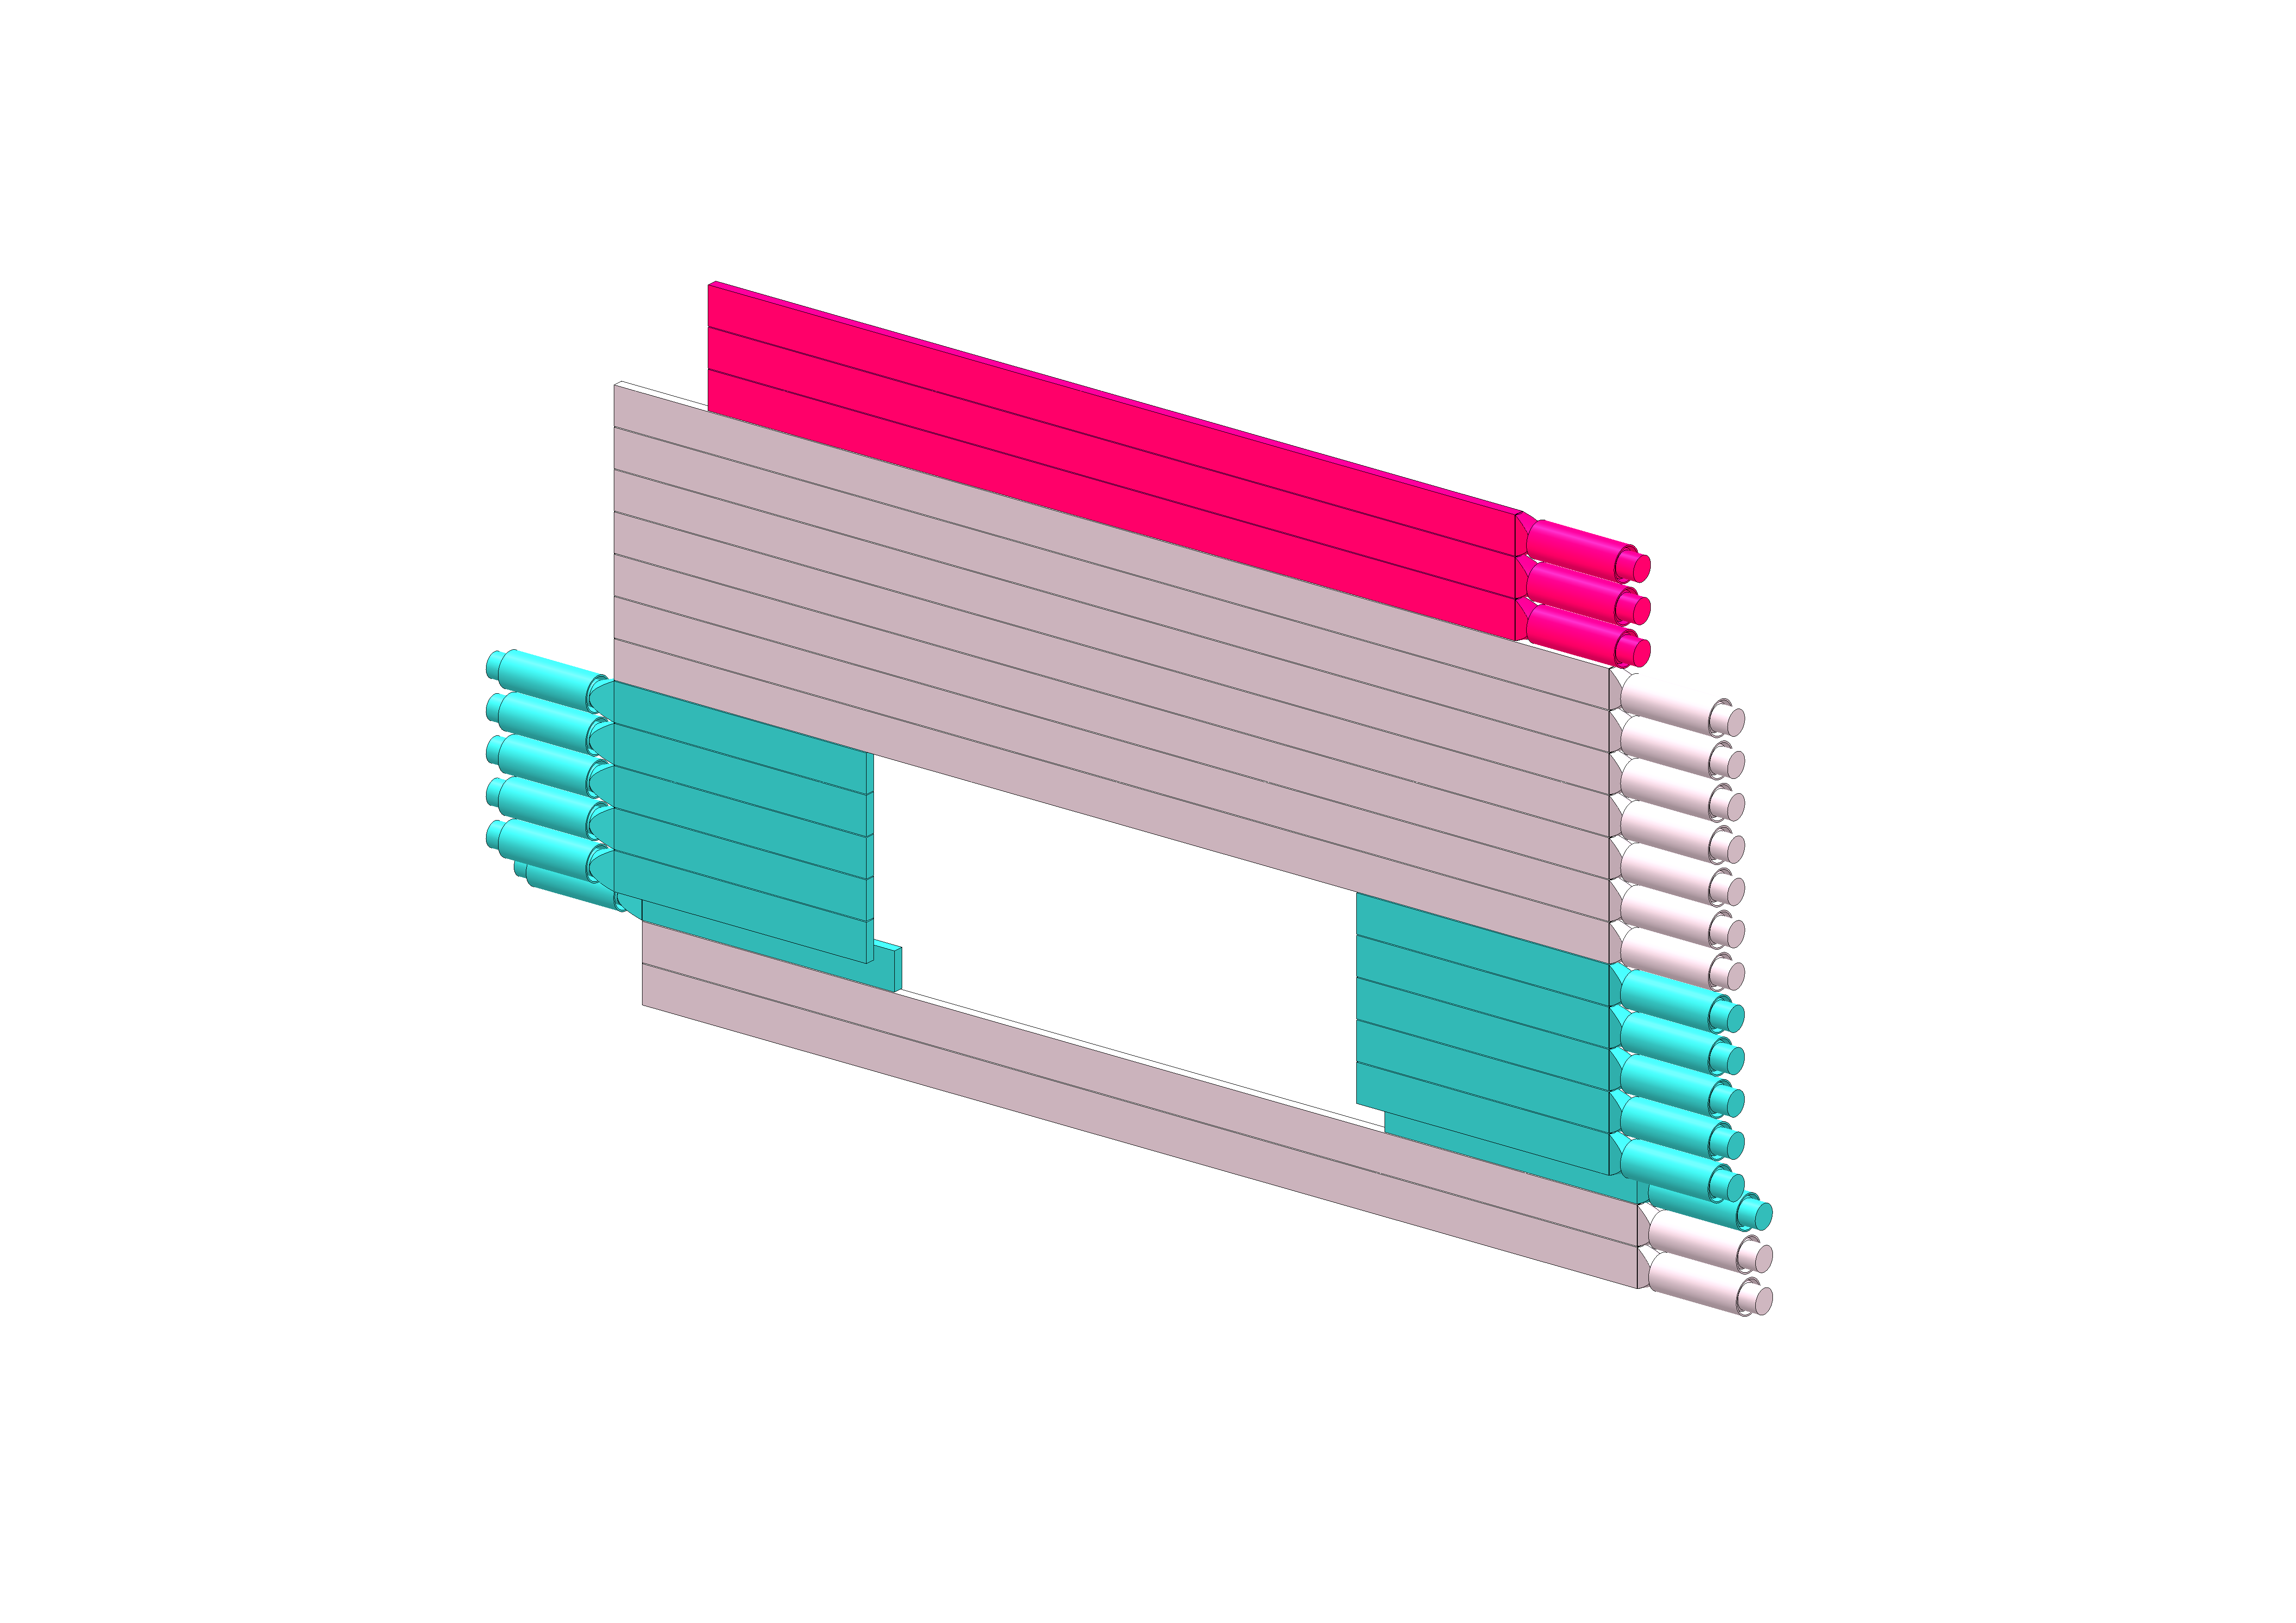
\includegraphics[width=0.48\textwidth]{VETO_DETECTOR_COLORED_2.png}
		\caption{BAND design. Need an updated nicer figure with direction of beam / coordinate system. Also have a similar 
		color scheme denoting the different sectors, so let's do a darker/ligher shade of green for the short bars so we can make 
		a table of sector, layer, ID, etc..}
		\label{fig:design}
\end{figure*}

{\color{red} ADD the different length of the bars here due to the constraint from beam pipe.}

\subsection{Components}
The timing resolution of the scintillator bars is impacted by many factors, and each component was optimized considering the design constraint and cost. Tests were 
performed varying the scintillant, reflective wrapping, photo-multipler tube (PMT), and optical-coupling-method of the scintillators to light-guides to PMTs to select the optimal combination

In our test measurements in  the lab, we used a coincidence setup between a ``test" scintillator bar and a ``reference" scintillator bar. Each bar has 2 PMTs 
coupled to the ends; the test bar has the PMTs which we wish to measure the time resolution. Both bars are wrapped in an optical reflector, and made light-tight 
via use of tape, coverings, and a black-box. The reference bar parameters are never changed during any measurement. A diagram of our test setup and electronics is shown in Fig. \ref{fig:test_stand}. The tested combination of components and results are summarized in Table~\ref{tab:tests}. 

The coincidence signal for our measurement is produced by a $^{60}$Co source which is placed between the two bars. $^{60}$Co undergoes $\beta^-$ decay to an excited state $^{60}$Ni, which then undergoes 
two $\gamma$ decays down to a $0^+$ ground state (1.17, 1.3 \si{\mega\electronvolt} respectively). The two $\gamma$-rays are collimated by two lead bricks to deposit the $\gamma$-rays at specific locations along the bars, allowing for the 
study of PMT time resolution as a function of distance from the PMT (or, due to attenuation along the bar, effective-energy observed by the PMT).

{\color{red}TO DO (Efrain): Discuss the results of the test and which PMT was chosen / why.}
Scintillator Material Reference \cite{scint-mat-ref}


\begin{table*}[t!]
	\caption{Tested configurations. Resolution given $2$ \si{\mega\electronvolt} energy deposit in middle of bar.}
	\begin{tabular}{  m{5em} | m{4em} | m{5em} | m{4em} | m{3em} |  m{5.7em} | m{3em} }
		\hline
			Scintillator & Reflector & PMT & Optical-coupling & Length (cm) & Cross section (\si{\centi\meter} x \si{\centi\meter}) & $\sigma$ (\si{\pico\second})\\
		\hline
		\hline
			EJ-200 & Al foil & ET-9214 & Grease & 200 & 7 x 7 & 270			\\
		
			EJ-200 & Al foil & R7724-10 & Grease & 200 & 7 x 7 & 240		\\
			EJ-200 & Al foil & R13435 & Grease & 200 & 7 x 7 & 300 			\\
		
			EJ-200 & Al foil & R13089 & Grease & 250 & 5 x 5  & 220			\\
			EJ-200 & Al foil & R7724-100 & Grease & 250 & 5 x 5 & 200 		\\
			
			BC-408 & XXX & ET-9214 & RTV 615 &50 & 7 x 7 & 150				\\
			BC-408 & XXX & R7724-10 & RTV 615 & 200 & 7 x 7 & 150			\\
		\hline
	\end{tabular}
	\label{tab:tests}
\end{table*}

\begin{figure*}[h!]
	\centering
	\begin{minipage}{0.48\textwidth}
		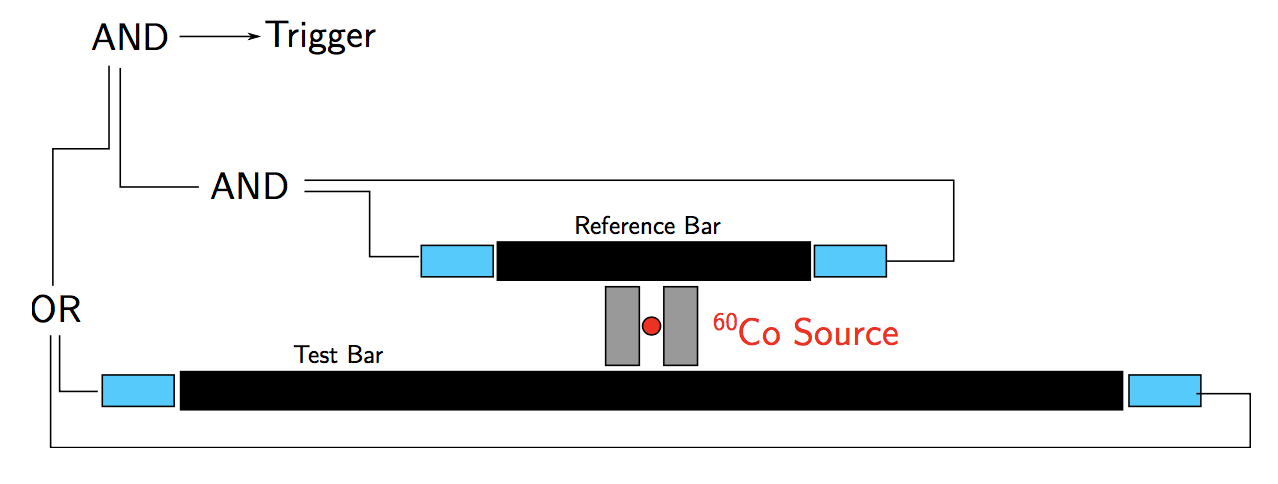
\includegraphics[width=\textwidth]{phys_setup.png} \\
		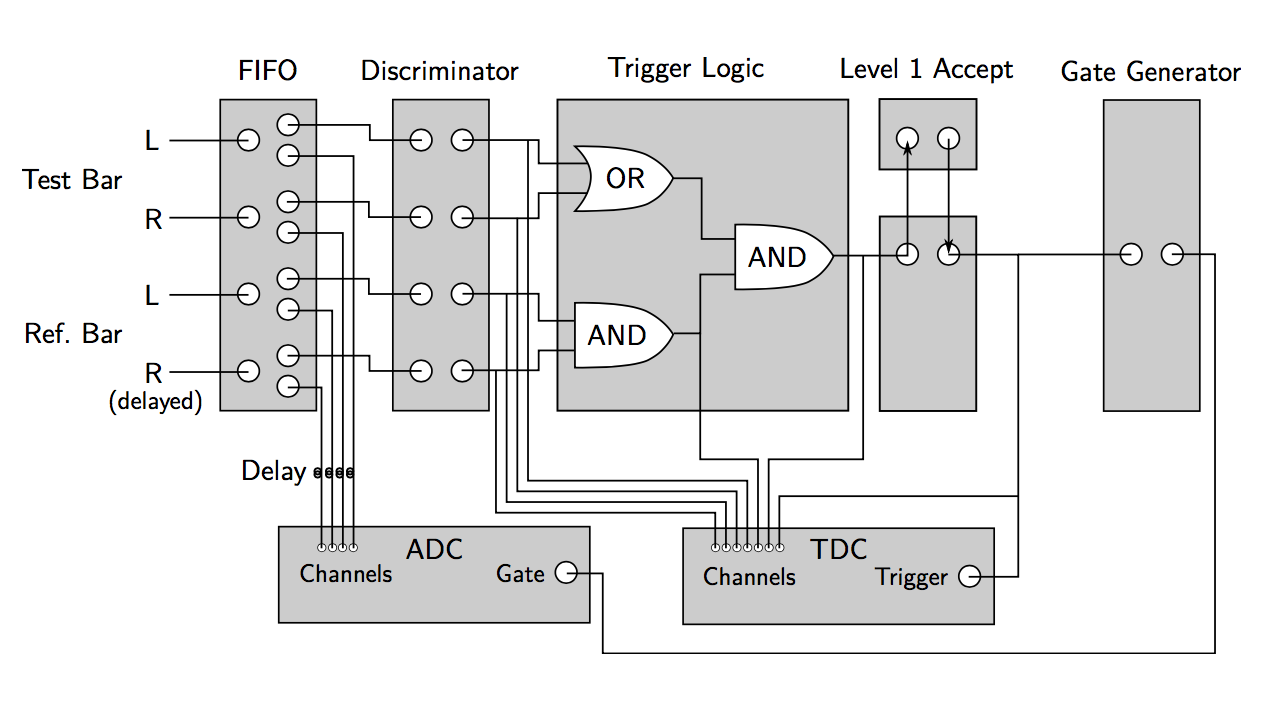
\includegraphics[width=\textwidth]{electr_setup.png}
	\end{minipage}
	\begin{minipage}{0.48\textwidth}
		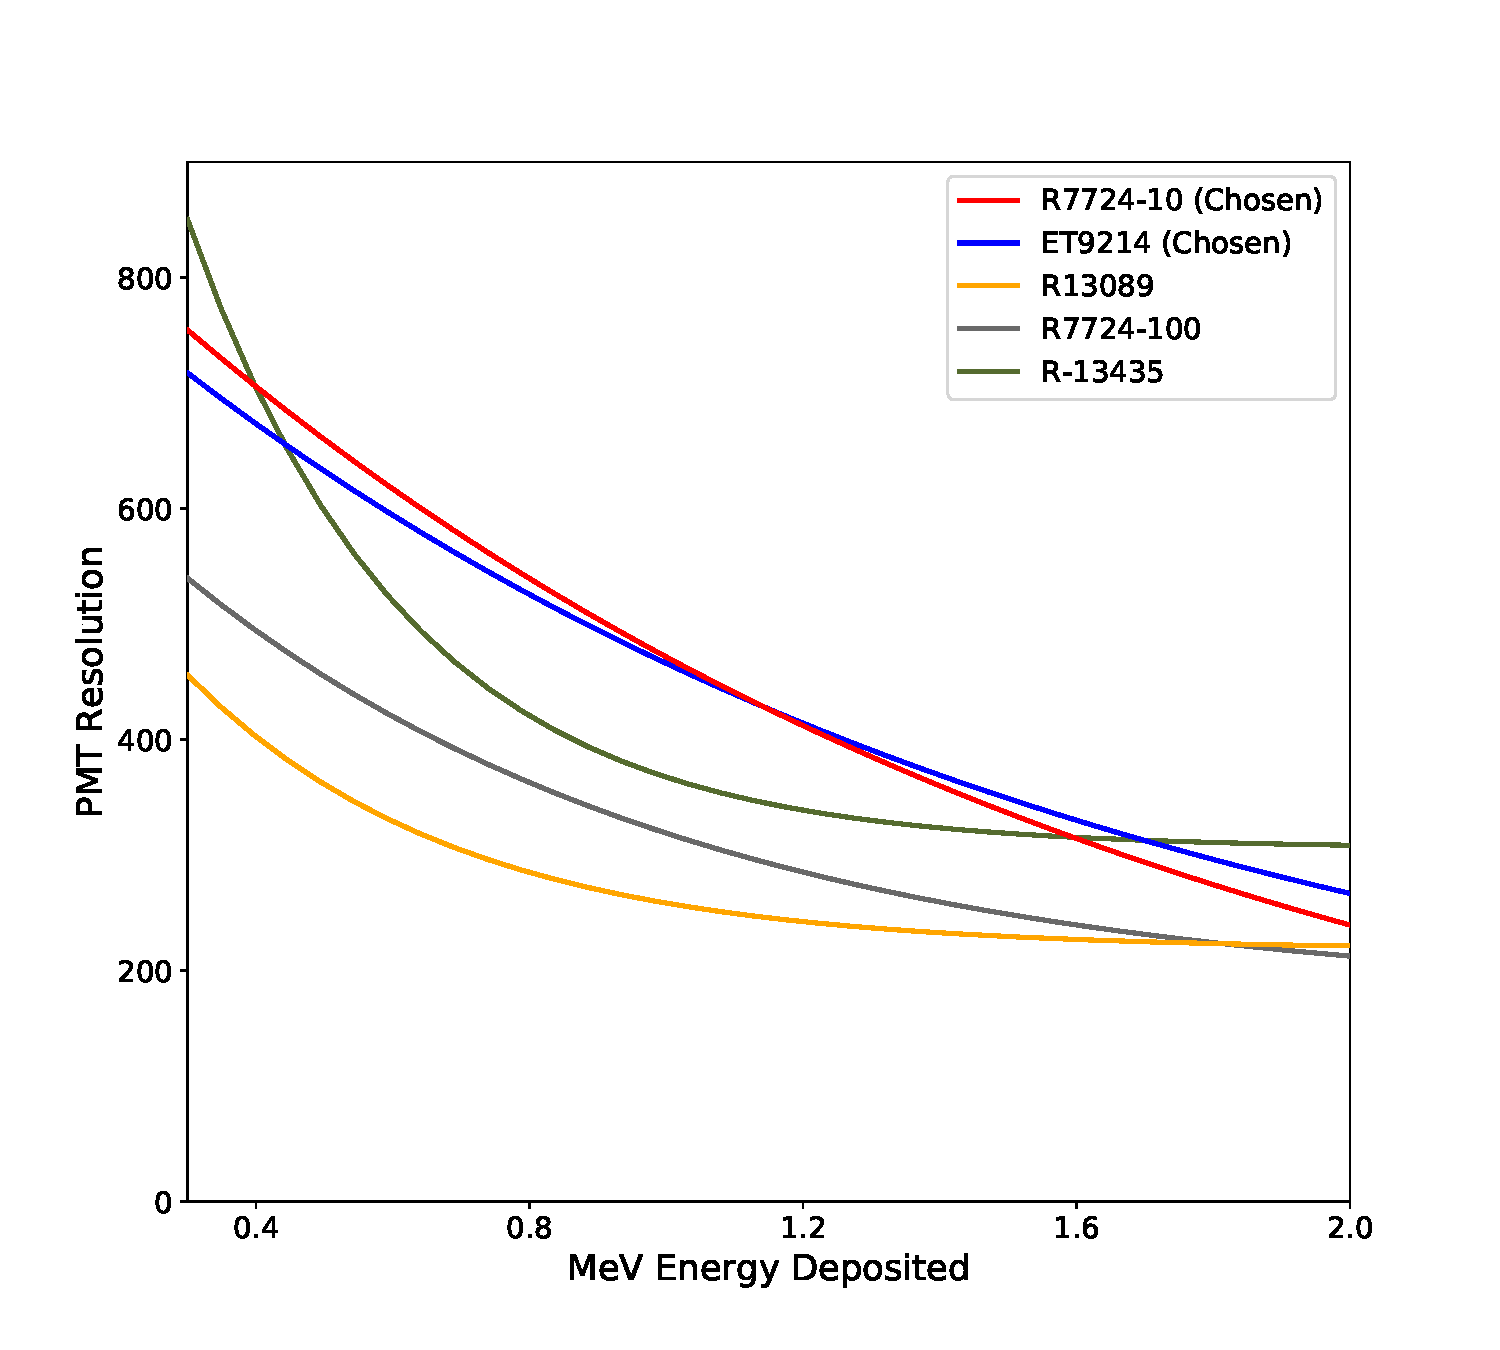
\includegraphics[width=\textwidth]{test-stand/test-resolutions.pdf}
	\end{minipage}
	\caption{Test to determine optimal choice of scintillant, PMT, optical wrapping and gluing material. Diagram of setup and electronics is shown on the left and obtained time resolution as a function of energy is shown on the right. The combination shown in blue and red was choosen for the }
	\label{fig:test_stand}
\end{figure*}

\subsection{Magnetic shielding}

Due to the placement of BAND in the fringe-field of the solenoid magnet of CLAS12 \cite{Fair:2020yfx}, all PMTs need a magnetic shielding. Testing of possible materials was conducted at Old Dominion University. 

{\color{red}TO DO: EDIT TEXT FROM KITTY AND ADD FIGURE WITH RESULTS:
We constructed a pair of 56-turn Helmholtz coils with a radius of 0.5 m, one borrowed from an existing setup, and one welded and wrapped on-site. We built an aluminium frame to maintain coil spacing, and laid a wooden platform between the coils. We also built a small prototype detector consisting of a 2 cm thick, 5 cm diameter disc of plastic scintillant, 7 cm long, 5 cm diameter cylindrical acrylic light guides, and PMTs with voltage dividers of the type we anticipated using to build the final detector. The disc of scintillant was mounted to the light guides with two-part optical cement, and the PMTs were mounted temporarily using optical grease. The detector was then light-proofed with Tedlar and stabilized in a simple cradle of PMT shipping foam. The cradle was placed on a stack of plastic shelving to center it in the field, then covered with black fleece.

As a baseline, the TDC and ADC peaks produced by strontium-90 and caesium-137 sources, and two different source placements were measured for a nominal operating voltage of the PMTs with no shielding. The goal was to place shielding such that the fewest number of events would be lost and the effect on timing would be minimized as magnetic field increased.

We tested two thicknesses of mu-metal shielding, each in two diameters, as well as two pipes of soft iron. The magnetic field, amount of detector covered by the shielding, the thickness of the shielding, the placement of two radioactive sources, and the angle of the detector to the field were all varied. The following table shows the full complement of variables:}

{\color{red}MISSING TABLE AND PIC FROM KITTY:}
%*only the caesium-137 was tested at 5 cm. The strontium-90 source triggered too few events when not directly atop the detector.

%Magnetic field: varied by changing current in the coils, limited to 80 gauss to prevent melting
%Angle: changed by aligning PMT cradle with markers on the magnet platform
%Cover: measured from PMT face, along light guides
%Shield thickness: varied by sliding one or both thicknesses of mu-metal shielding over the PMTs. Soft iron was only tested alone.
%--------

The results show that a xx thick $\mu$-metal shielding placed 5 cm past the PMT faces is most effective to preserve events and minimize timing distortions. Therefore, every PMT in the detector has been equipped with such a shielding. During installation, we ensure that the $\mu$-metal is also covering an area of the light guide in front of the PMT photo cathode to obtain optimal shielding.

\subsection{Lead shielding}
To minimize background from backward going photons, a lead wall was installed between the target of CLAS12 and BAND. This lead wall consists of individual 20 \si{\milli\meter} thick blocks stacked in front of the veto layer. Each block is covered on both sides with an Aluminium layer to simplify the handling of every block. We estimated a reduction of the background rates from photons by xx. {\color{red} more details here or not?}

%%%%%%%%%%%%%%%%%%%%%%%%%%%%%%%%%%%%%%%%%%%%%%%%%%%%%%%%%%%%%%%%%%%%%%%%%%%%%%%%%%%%%%%%%%%%%%%%%%%

%\section{Description}

%%% ----------------- Geometry subsection
%\subsection{Geometry}

%%% ----------------- Components subsection
%\subsection{Components}

%\begin{table}[t!]
%	\caption{}

%	\label{tab:tests}
%\end{table}

\subsection{Laser Calibration system}
Due to the placement of the BAND, in CEBAF 12 \si{\giga\electronvolt} with the CLAS12 magnetic fields \cite{Fair:2020yfx} there is a lack of high-rate exclusive processes 
that can be used for monitoring performance stability and perform calibrations. A laser system \cite{band-laser} was implemented to validate performance during data-taking. This system also 
provided a method to quickly perform various calibrations (discussed below). For this purpose every bar in BAND was equipped with an optical fiber which was connected via a patch panel to the optical/fiber splitter of the laser system. A reference signal of the laser system is provided by a photo diode. The output signal of the photo diode is inverted and shaped before it is sent to the BAND read-out system. The signal is detected by the same ADCs and TDCs which are used for the PMT signals.


%%% ----------------- Electronics subsection
\subsection{Electronics and DAQ}
In the experiment, the high voltages for each PMT (typically in the range of 1500 V) are provided by a multi-channel CAEN SYS4527 mainframe with 11 A1535SN cards (24 channel each).
A schematic drawing of the read-out electronics and its components is shown in Fig. \ref{fig:electronic-diag}. The signal of each PMT is split to measured ADC and TDC independently. 
The signal splitters are custom made and have been used in previous experiments at Jefferson Lab (COULD ADD REF to HPS herenwhere it was used before).
From the splitter one signal is sent to flash-ADCs (250 VXS, 16 channels/board, made and owned by Jefferson Lab \cite{fadc-manual}) while the other signal is sent to  discriminators (16 channels/board, also made by Jefferson Lab [ADD REF, possibly online]).
The discriminated time signal goes to a TDC (CAEN VX1190A, 128 channels/board, 100 ps/channel resolution). 
In total, the system consists of 16 flash-ADCs in one VXS crate, 16 discriminators and a TDC in a VME crate and 16 splitters.  Furthermore, a trigger signal distribution card for the flash-ADCs and trigger interface boards are installed in the crates. All components are part of the standard electronics components of CLAS12 at Jefferson Lab \cite{clas12-daq, clas12-trigger}.

The detector read-out is either triggered by the main trigger system from CLAS12 or by stand-alone detector triggers for tests and calibrations with cosmics, radioactive sources and the laser system. The stand-alone triggers are implemented by a programmble logic board (CAEN V1495, ADD REF to webpage) and they consist of a single bar trigger for source measurements and a coincidence bar trigger for cosmics and laser measurements. The later one is also feed to the central CLAS12 trigger system to allow monitoring of the detector by recording laser hits during real data taken. This special trigger rate is usually about 10 \si{\hertz} compared to the $\approx$ 15-20 \si{\kilo\hertz} trigger rate from electron interactions in the target.


\begin{figure*}[h!]
	\centering
		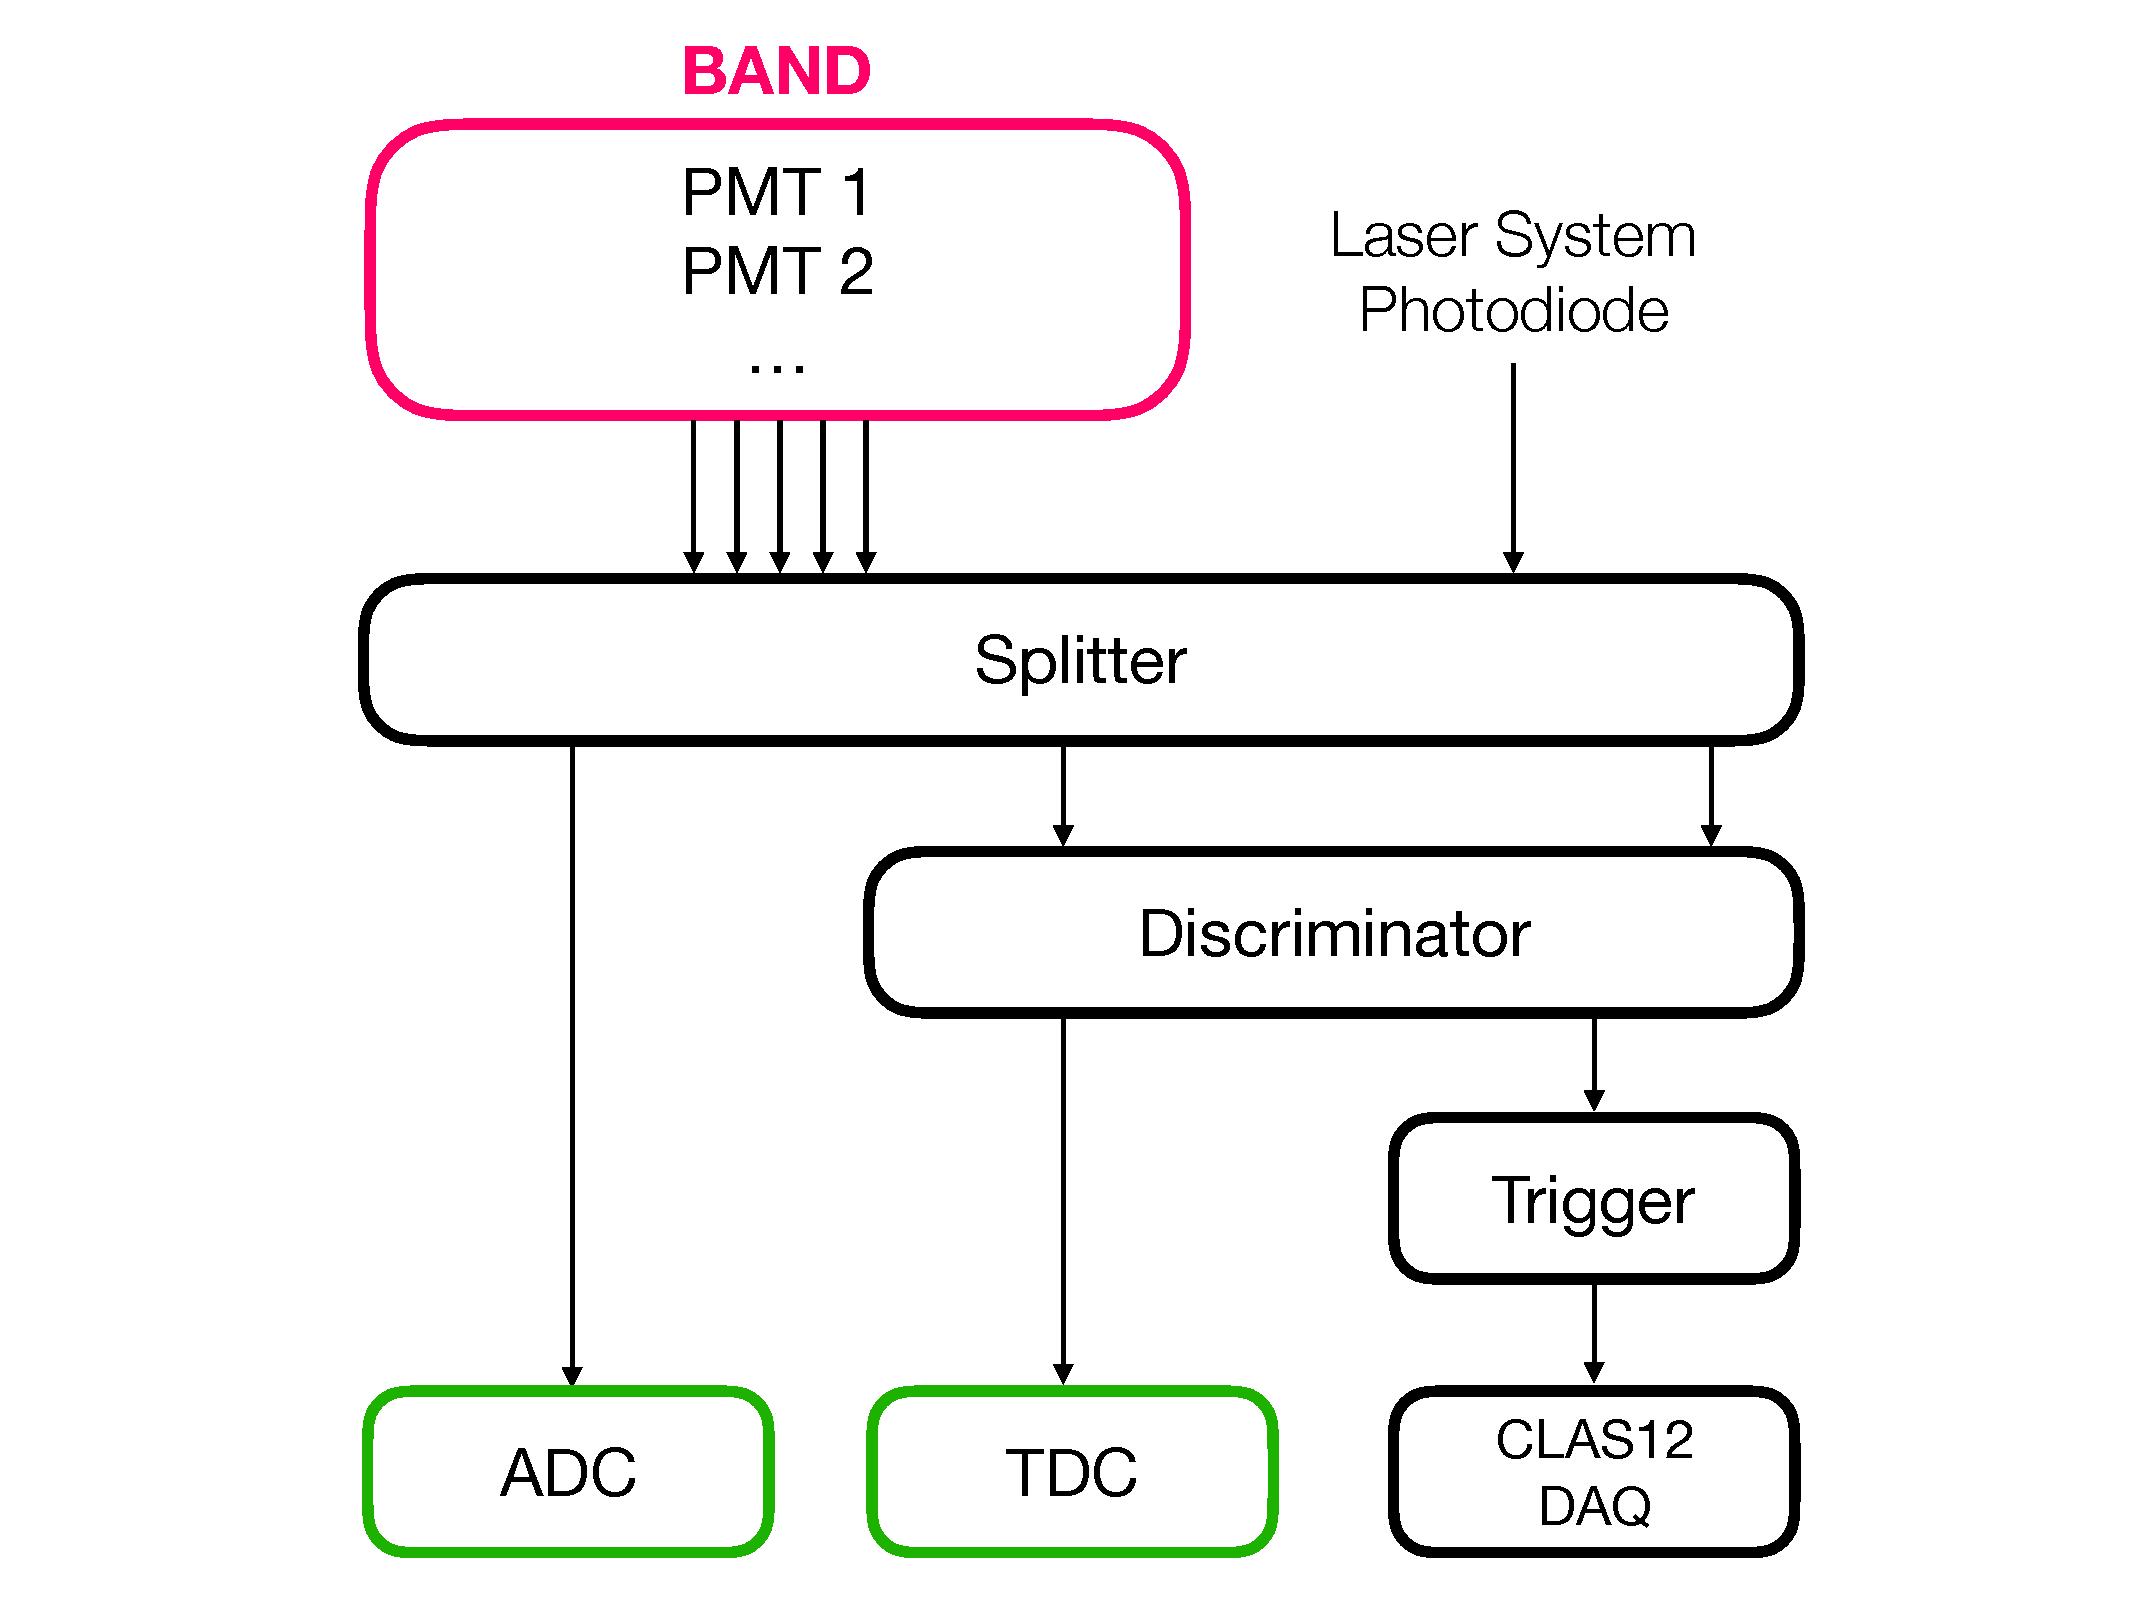
\includegraphics[width=0.96\textwidth]{figures/electronics-diag.pdf}
	\caption{Electronic schematic of the BAND read-out. Every PMT signal is split and ADC and TDC information are obtained. Additional outputs of the discriminators are used to create single bar and cosmic-laser triggers from BAND.}
	\label{fig:electronic-diag}
\end{figure*}


%%% ----------------- Assembly subsection
\subsection{Final Assembly}
{\color{red} Shall we keep this section describing some remarks on the final assembly and having 1-2 nice pictures or scratch it?}
%%%%%%%%%%%%%%%%%%%%%%%%%%%%%%%%%%%%%%%%%%%%%%%%%%%%%%%%%%%%%%%%%%%%%%%%%%%%%%%%%%%%%%%%%%%%%%%%%%%


\section{Performance}
%%% ----------------- Gain matching subsection
In this chapter, we first describe the performance of every bar and the necessary calibration steps to achieve it. Especially, a set of timing calibrations is necessary to achieve the required time of flight resolution of better than 300 \si{\pico\s}.
In the second part of the chapter, the performance of the whole BAND detector is shown with a focus on neutron identification and efficiency.
\subsection{Individual bar performance}
\subsubsection{Gain matching}
{\color{red} Should we add more detaill like FTOF does -- what value for cosmic did we match to / why...?}
In order to have similar response to a given energy deposit across all PMTs of BAND, each PMT's HV was optimized using
cosmic rays. Multiple data sets with varying PMT HV were taken with cosmic rays, and combined to produce a gain curve for 
each PMT. A typical ADC spectrum from cosmic data for a single HV setting %and the resulting gain curve from fitting the 
%cosmic peak from many HV settings are both shown
is shown in Fig~\ref{fig:gain}. The resulting HV settings across all PMTs in BAND is 
shown in Fig~\ref{fig:hv_settings}. The spread of the settings for the short bars (red points) stems from a non-uniform behaviour from the ET9214 PMTs which were installed on the short bars. The Hamamatsu R7724-10 PMTs show are more uniform gain performance.
\begin{figure*}[h!]
	\centering
		\begin{minipage}{0.48\textwidth}
			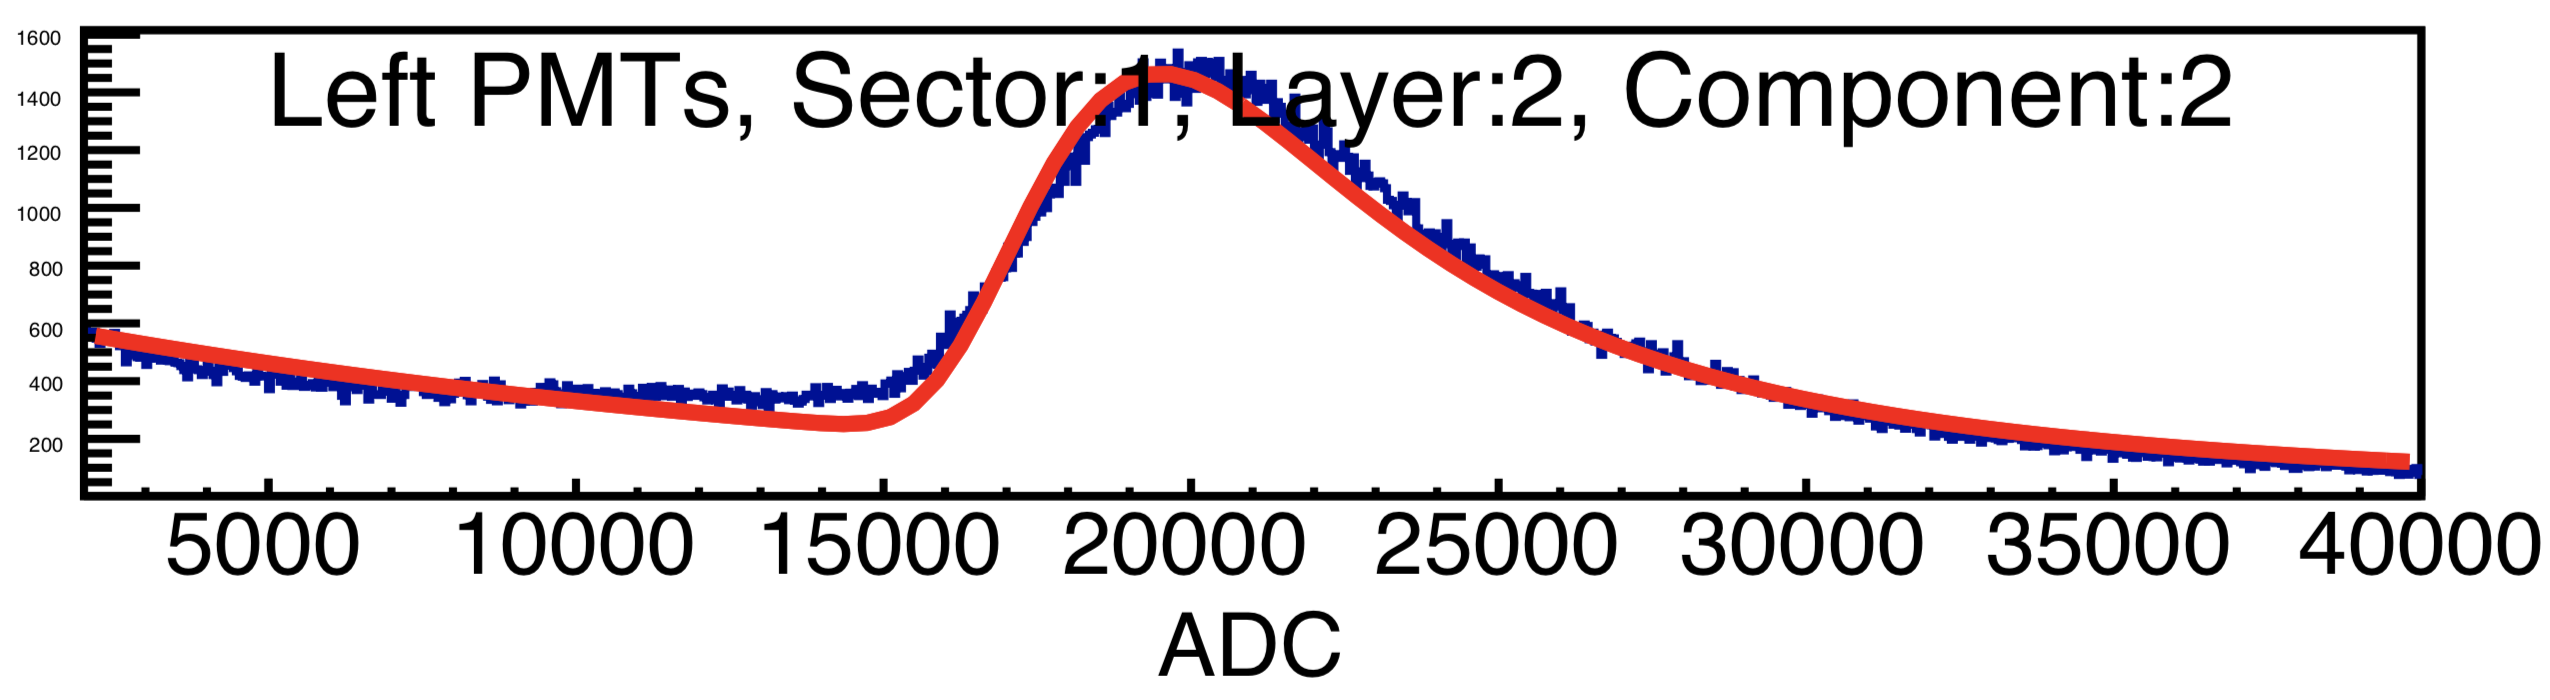
\includegraphics[width=\textwidth]{adc-spectra.png}\\
			%\includegraphics[width=\textwidth]{.png}
			\subcaption{}
			\label{fig:gain}
		\end{minipage}
		\begin{minipage}{0.48\textwidth}
			\includegraphics[width=\textwidth]{hv-settings.pdf}
			\subcaption{}
		\label{fig:hv_settings}
		\end{minipage}
		\caption{Gain matching of BAND PMTs. (a) Typical ADC spectrum for a PMT with cosmics. (b) All PMT HV settings for similar gains. One sees a greater 
		spread of HV needed to match gains in the short bars which have ET9214 PMTs.}
\end{figure*}


%%% ----------------- Energy deposit subsection
\subsubsection{Energy deposit calibration}
The ADC response of each PMT is converted to \si{\mega\electronvolt} energy deposition by measuring the response to 
multiple radioactive sources. The sources $^{60}$Co, $^{22}$Na, $^{137}$Cs were chosen due to the gamma rays that have 
Compton edges of $0.963$ and $1.118$, $0.477$, and, $1.062$ and $0.341$, respectively (in \si{\mega\electronvolt}). The 
response to each source was measured in the center of the bar. Using the ADC response to all sources, in combination with the 
attenuation length of the bar, the ADC response can be converted to \si{\mega\electronvolt}.

A typical response of a PMT to  $^{60}$Co is shown in Fig.~\ref{fig:mev_conversion} (left), along with the extracted Compton edge for a 
number of bars (right). The edge has been fitted by a parametrization desribed in {ADD REF]. The extracted Compton edges for various bars are quite similar which also shows the a good gain matching obtained with cosmics. 
{\color{red} Should we add more details here? Like results from all sources and a fit for the conversion? At Efrain: Didn't we use actually geometric mean and not single PMT fits?}

\begin{figure*}[h!]
	\centering
		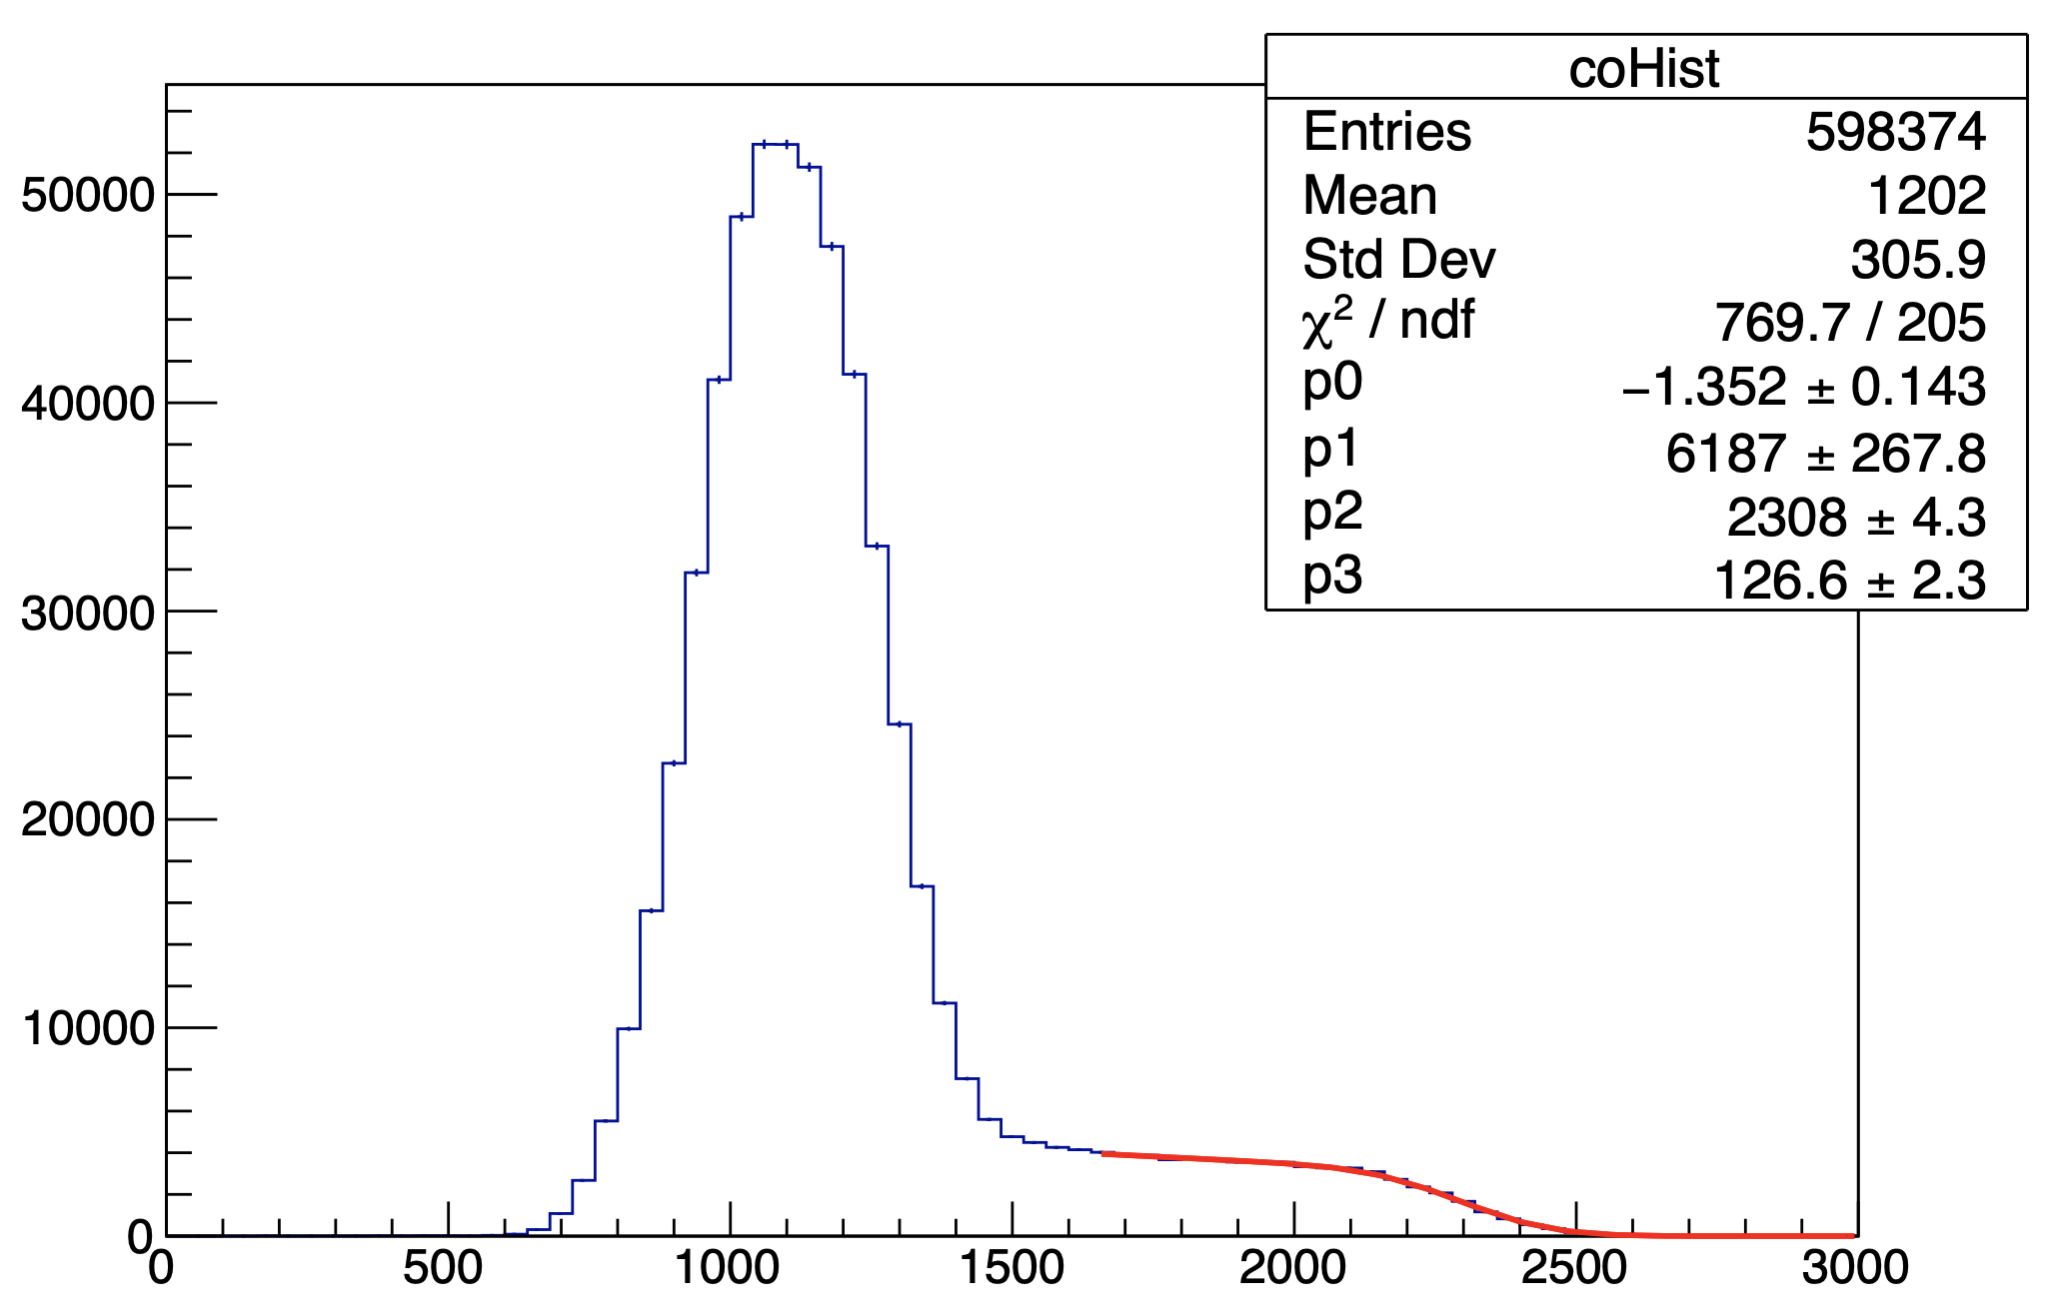
\includegraphics[width=0.48\textwidth]{co-compton.png}
		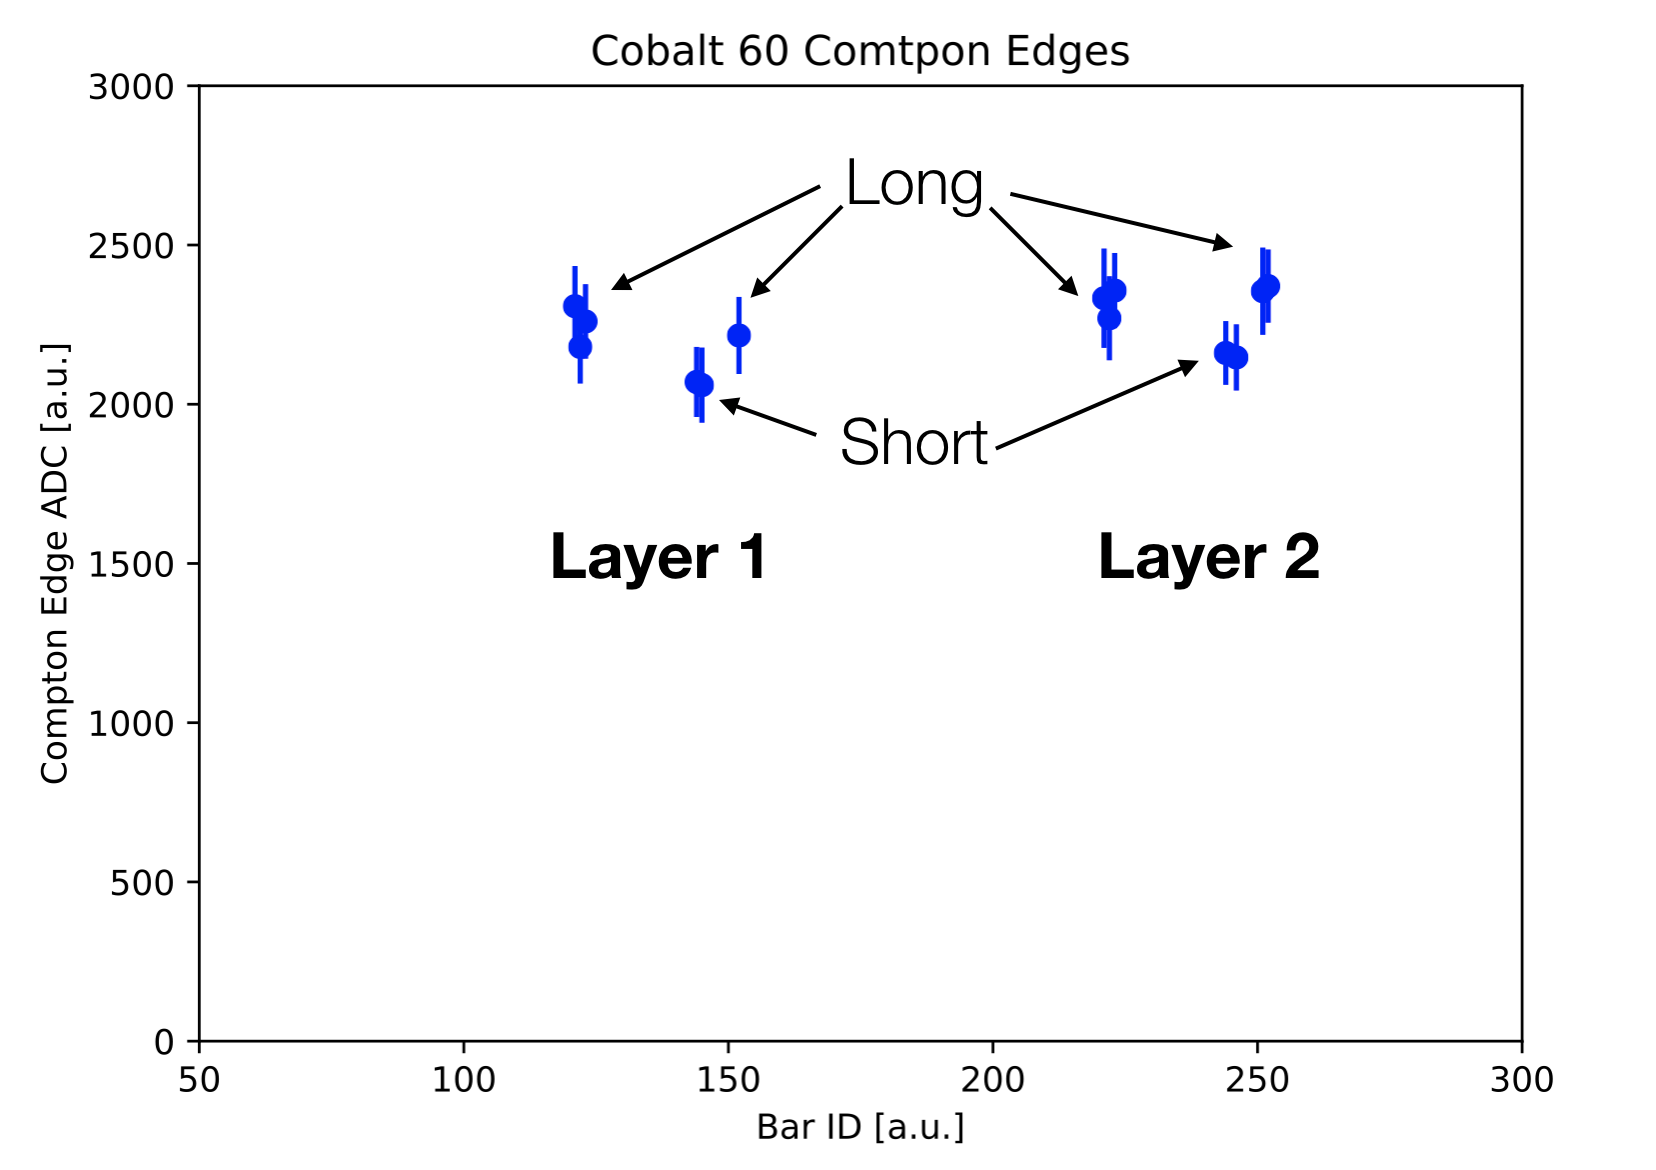
\includegraphics[width=0.48\textwidth]{coedges.png}
	\caption{Left: ADC spectrum for a $^{60}$Co placed on the center of the bar along with the fit of the Compton edge. Right: Obtained Compton edge for different bars.}
	\label{fig:mev_conversion}
\end{figure*}

%%% ----------------- Time-walk subsection
\subsubsection{Time-walk calibration}
Time-walk calibrations were performed with the laser system \cite{band-laser}. A motorized fiber optic attenuator is used to vary
the amount of light delivered to each bar. Waveforms and times are measured as the attenuator scans from $40$ \si{\decibel} to $0$ 
\si{\decibel}. Time-walk curves and calibrations are taken per PMT. The laser pulse, immediately after fiber-coupling, is initially 
split with $90\%$ going to the attenuator, and $10\%$ going to a photodiode used as a reference time for any calibrations 
performed with the laser system.

Dependence of a typical PMT time to pulse height is seen in Fig.~\ref{fig:time_walk} (left). To correct for time-walk, we parameterize 
this dependence on pulse height, $A$, as:
\begin{eqnarray}
	\begin{split}
		t_*(A)	&= \alpha + \frac{\beta}{\sqrt{\textrm{A}}}.				
		\label{eqn:time_walk}
	\end{split}
\end{eqnarray}
The residual after time-walk correction, $t-t_*$, is shown in Fig.~\ref{fig:time_walk} (right). At pulse heights close to threshold, the 
parameterization is not flexible enough and under-estimates the strong dependence on pulse height. However, signals with pulse 
heights this low are not of interest, as a software cut on minimum energy deposition is needed to improve signal-to-background 
which removes these pulses (discussed in Section {\color{red}4.2.3}).

\begin{figure*}[h!]
	\centering
		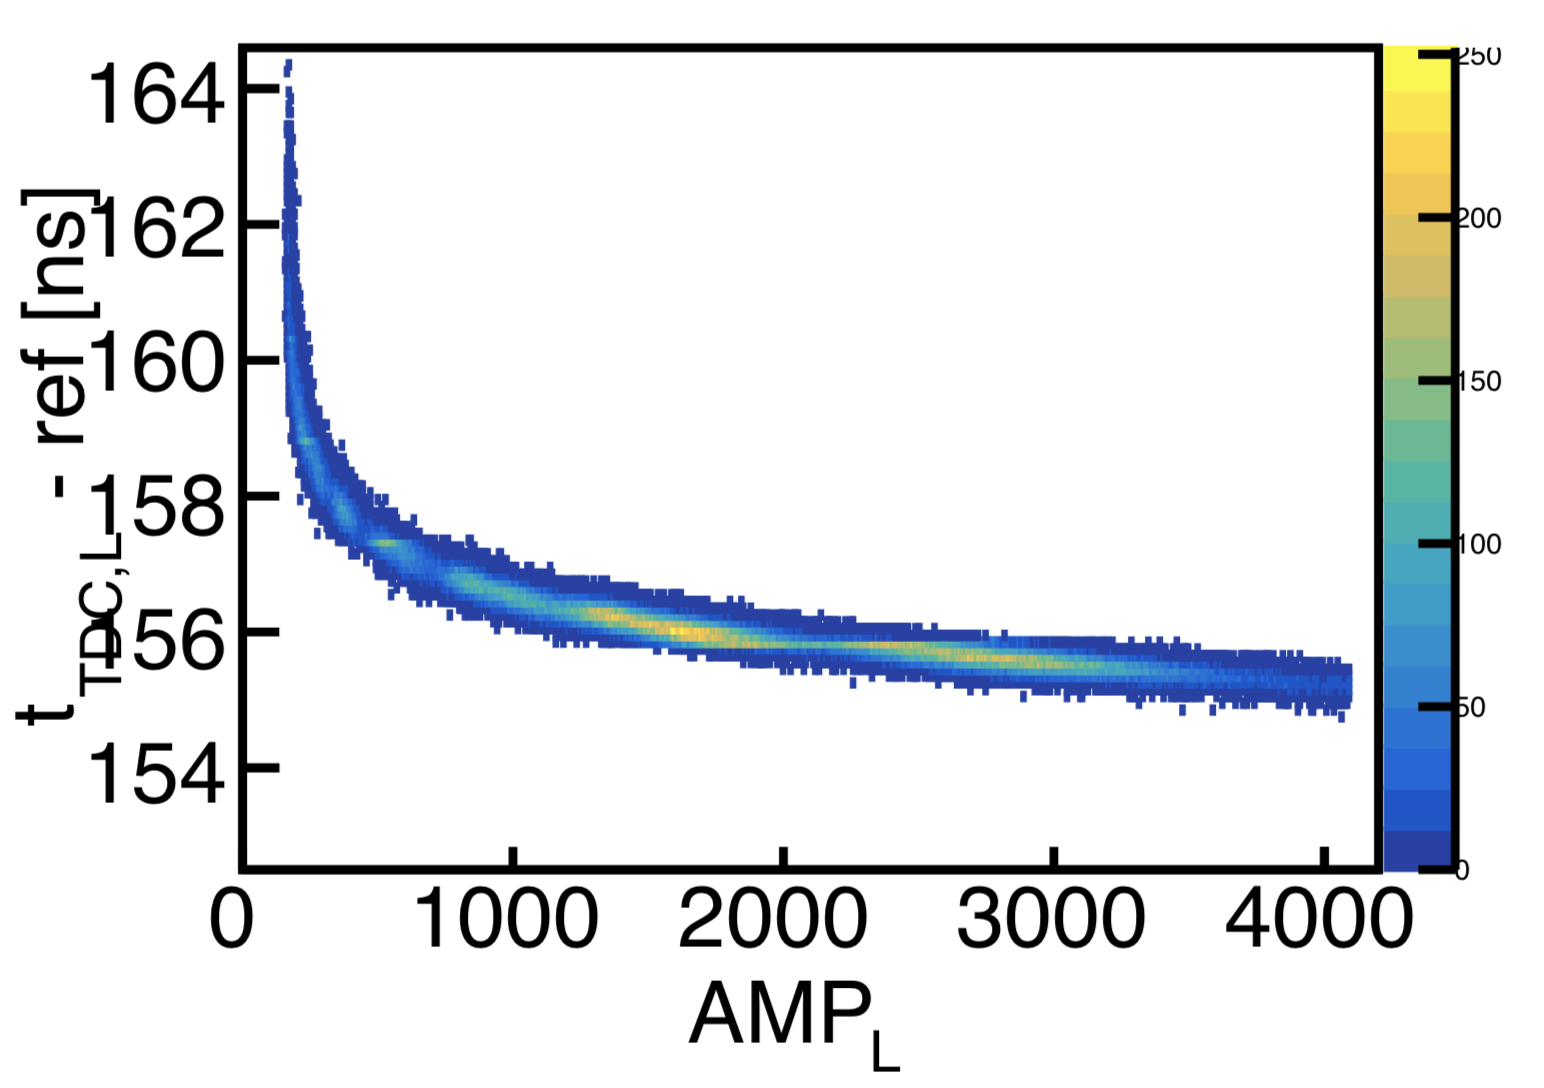
\includegraphics[width=0.48\textwidth]{tw_before.png}
		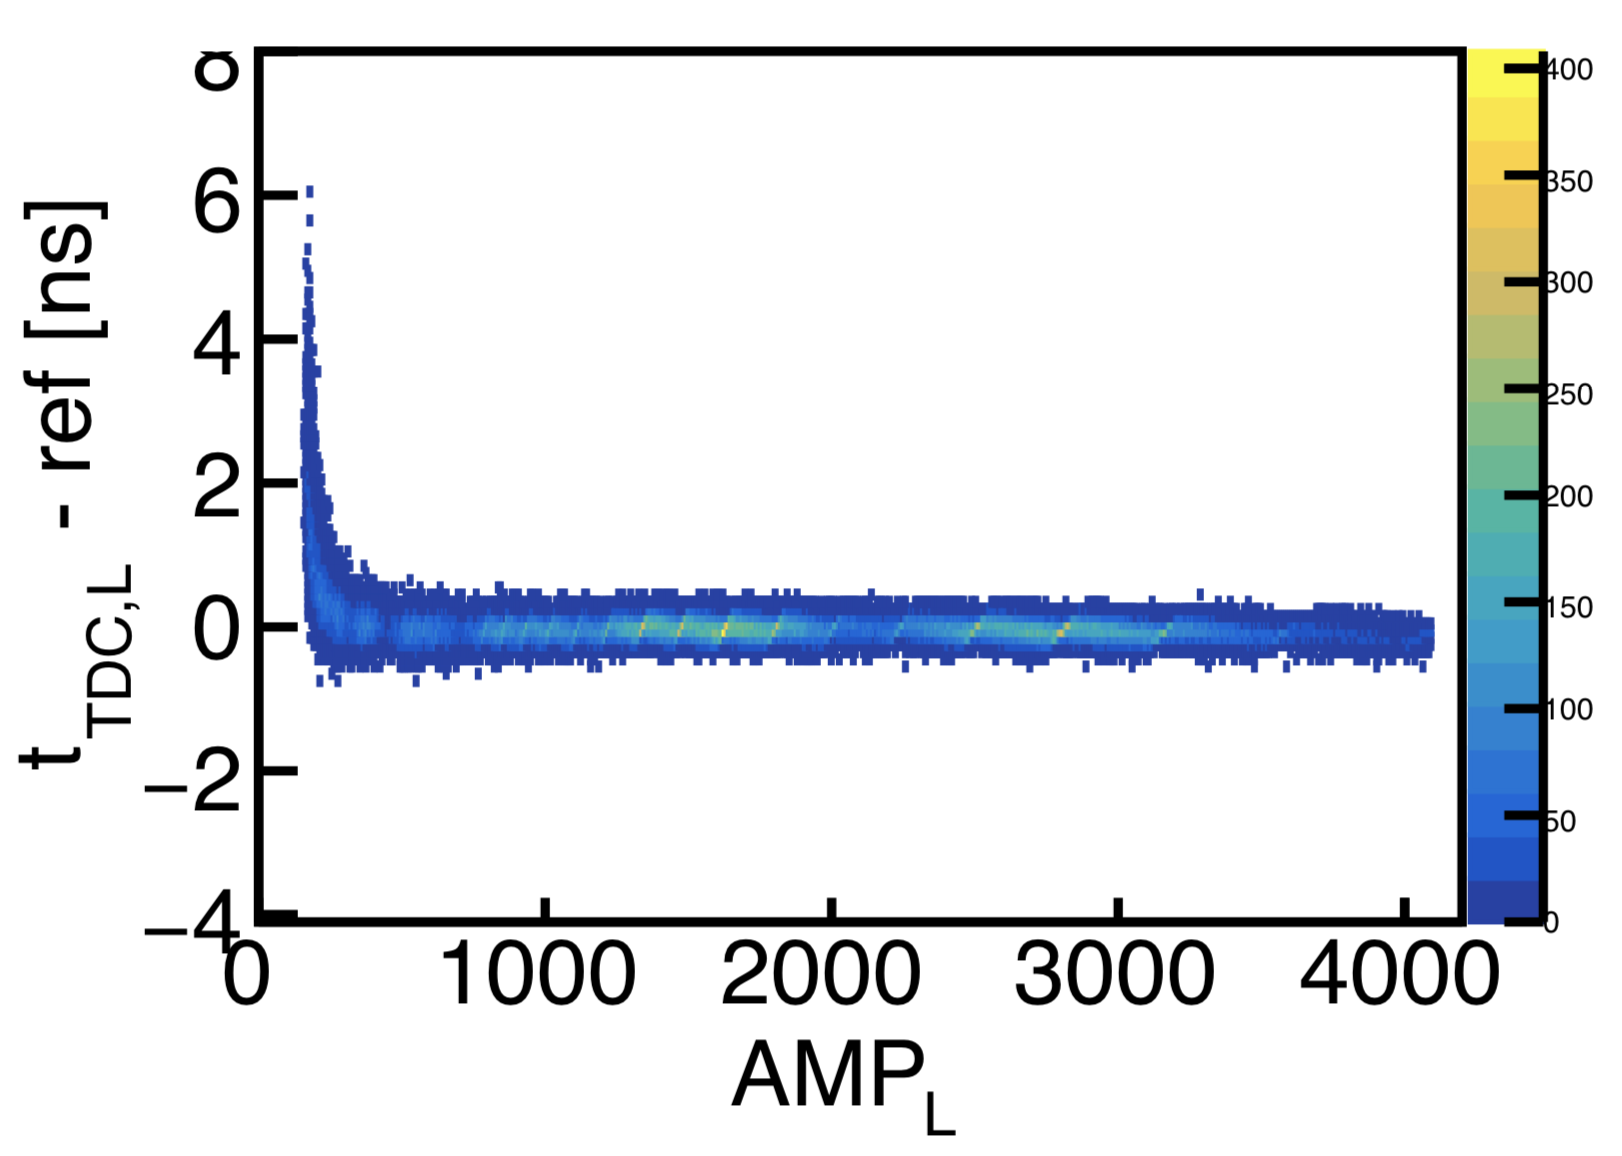
\includegraphics[width=0.48\textwidth]{tw_after.png}
	\caption{Time-walk calibration: Typical time to pulse height spectrum for one PMT with respect to the time for the reference photodiode before time-walk correction (left) and after time-walk correction (right).}
	\label{fig:time_walk}
\end{figure*}

%%% ----------------- Effective velocity subsection
\subsubsection{Effective velocity}
The relative time delays between PMTs on the same bar, and the speed-of-light in that bar, are extracted using cosmic ray 
data after time-walk calibrations are done for each PMT. The width of the relative timing distribution between the left and 
right PMT on a given bar is used to extract the effective velocity in a bar knowing the length of the bar,
\begin{eqnarray}
	\begin{split}
		t_L - t_R 	= -\frac{2x}{v}							\\
		 -\frac{L}{v}	\leq 	t_L - t_R 	\leq \frac{L}{v},				
		 \label{eqn:eff_vel}
	\end{split}
\end{eqnarray}

and the relative time offset is given by the center of the distribution (see Fig.~\ref{fig:eff_vel} left). The obtained effective velocities for each bar are shown in Fig.~\ref{fig:eff_vel} (right) distinguished between short bars (red) and long bars (blue). The observed difference is due to geometrical effects from the different bar length.

\begin{figure*}[h!]
	\centering
		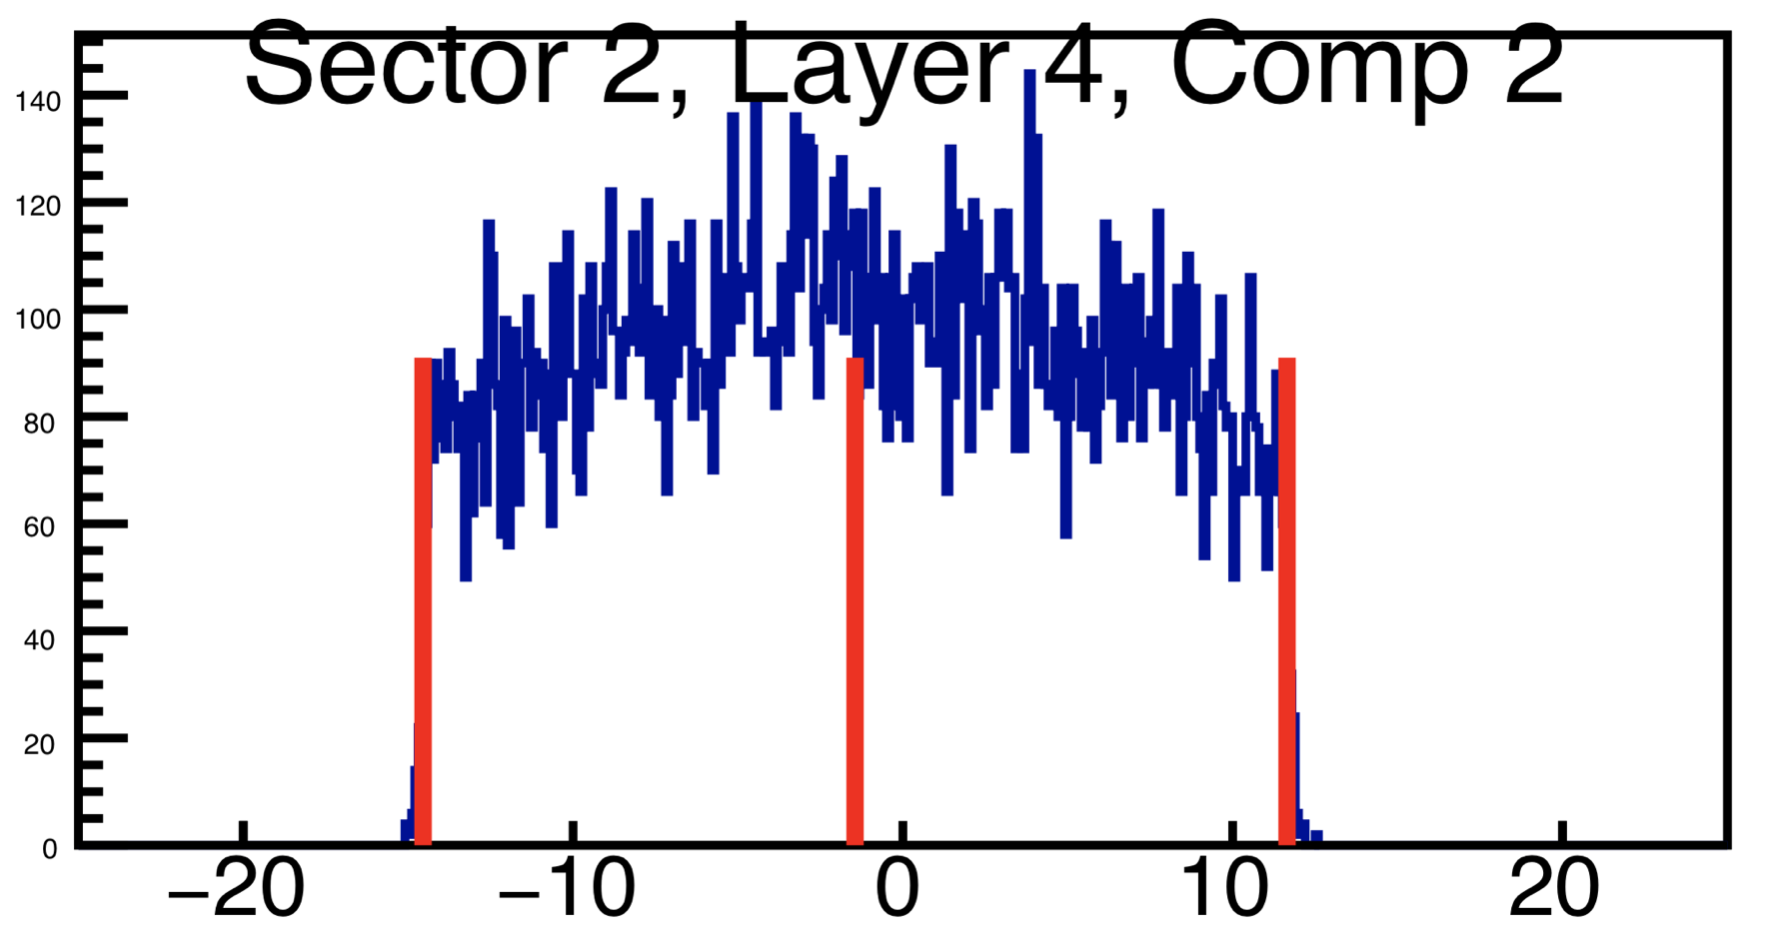
\includegraphics[width=0.48\textwidth]{lr_eff_vel.png}
		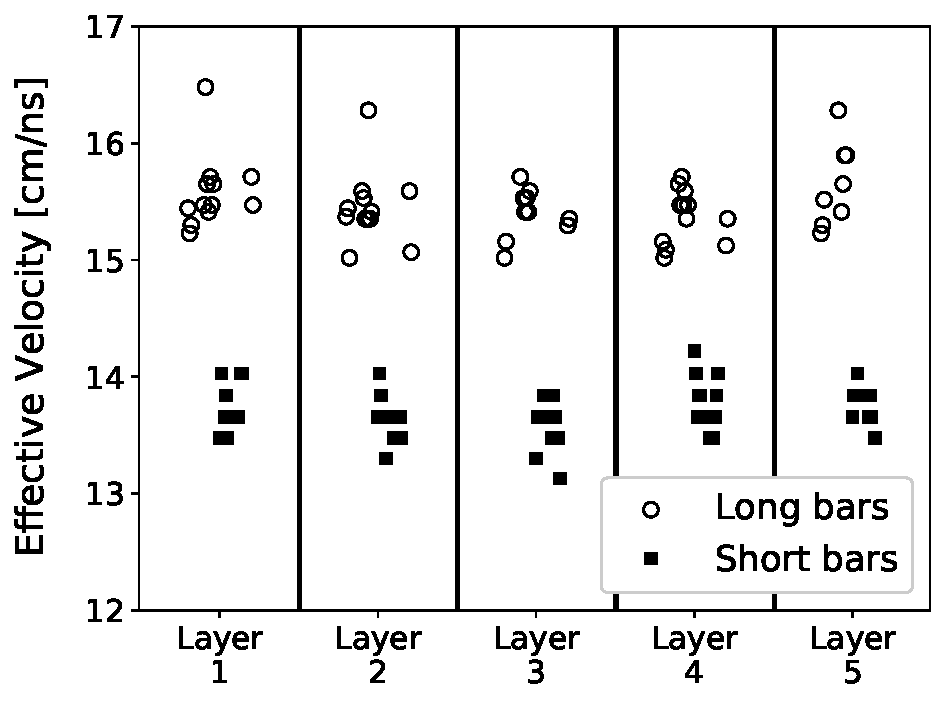
\includegraphics[width=0.48\textwidth]{eff_vel.pdf}
	\caption{Effective velocity: Left-Right time spectrum in a single bar after time-walk correction for every PMT (left). Obtained effective velocities for each bar (right). The differences in effective velocities between long bars (blue) and short bars (red) are probably due to geometrical effects from the different bar length.}
	\label{fig:eff_vel}
\end{figure*}

%%% ----------------- Attenuation length subsection
\subsubsection{Attenuation length}
The attenuation length of the scintillator material can be extracted using cosmic ray data by using the 
amplitude ($A$) and time measured by both PMTs in the bar:
\begin{eqnarray}
	\begin{split}
		A_L(x) &= A_0 e^{-\frac{1}{\mu}\left(L/2-x\right) }				\\
		A_R(x) &= A_0 e^{-\frac{1}{\mu}\left(L/2+x\right) }				\\
		R(x) \equiv \ln{\frac{A_L(x)}{A_R(x)}} &= \frac{2x}{\mu},					
		 \label{eqn:atten}
	\end{split}
\end{eqnarray}
where $x=-\frac{v}{2}(t_L - t_R)$. So by measuring the slope of $R(x)$, one can extract the attenuation length 
of the bar. See Fig.~\ref{fig:atten} (left) for the typical response of a bar to cosmic ray data, and the resulting attenuation 
length obtained from the central part of the bar (right). The plateau shape of the amplitude ratio closer to the edge of the bar is probably induced by reflections at the light guides.   
 {\color{red} A comparison of the attenuation lengths of all bars can be seen in Fig.~\ref{fig:atten_allbars} }.
 {\color{red} Shall we add more details?  Comparision how does it look with the ADC integral? }.
\begin{figure*}[h!]
	\centering
		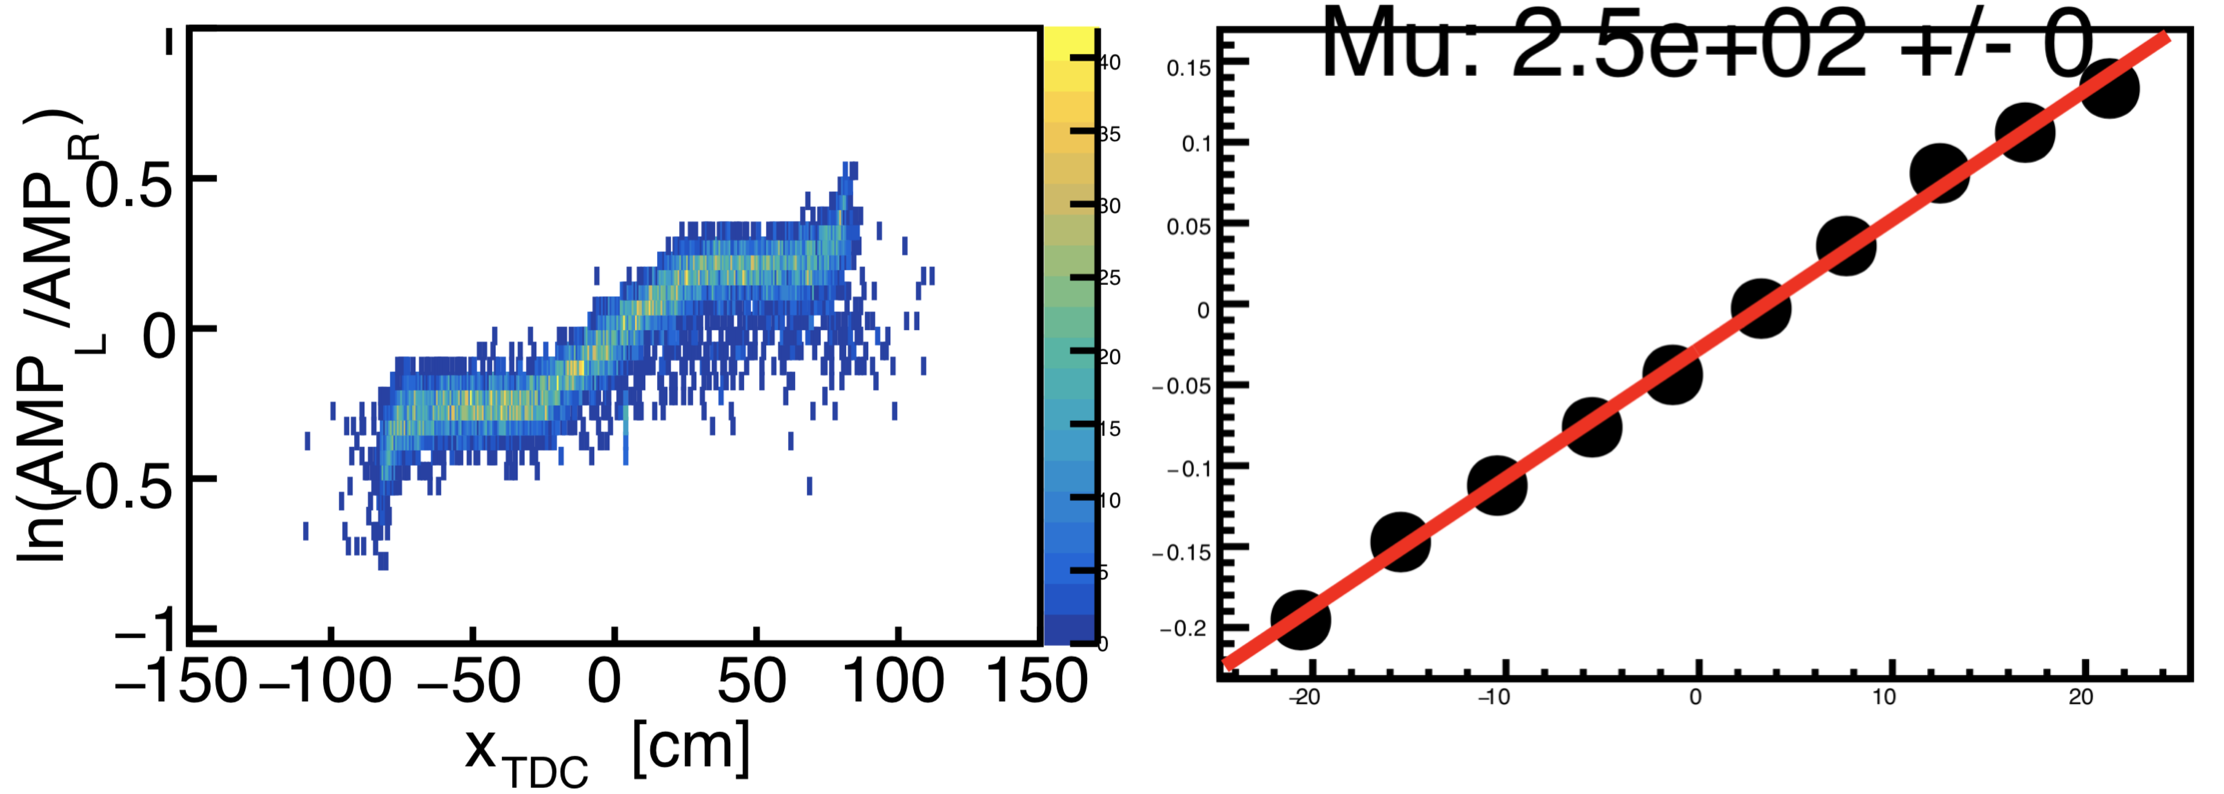
\includegraphics[width=0.96\textwidth]{atten.png}
	\caption{Left: Log ratio of amplitudes from both PMTs on a bar as a function of position along the bar (positive x is left side of the bar). Right: Linear fit of left plot in the center of the bar to determine the attenuation length.}
	\label{fig:atten}
\end{figure*}

%%% ----------------- Bar offsetts subsection
\subsubsection{Individual Bar offsets}
After all bars are individually calibrated, relative time delays between bars can still remain, and require correction to combine 
statistics from all bars. The alignment of all bars can be done quickly using the laser calibration system, as the laser pulse arrival 
time to each bar should be within timing resolution, provided all of the fiber optic cables are of the same length to the BAND bars. 
However, the $51$ \si{\centi\meter} bars have fiber optic cables of $1.5$ \si{\meter} length from the patch panel to the center 
of the bars, and the $160$ and $200$  \si{\centi\meter} bars have fiber optic cables of $2.5$ \si{\meter} length. This residual offset 
between the ``short" bars and ``long" bars can be corrected later by using the photon arrival time to the bars with production data, 
grouping the short bars and long bars separately (see later). Furthermore, obtaining bar alignment with only production data 
requires high-statistics datasets due to the backward-angle placement of the BAND. 

Using data taken with the laser calibration system, bar alignment is done on the average time of a given bar, 
$t_{avg,i} = \frac{1}{2} \left(t_L + t_R\right)_i$. An offset is extracted for each bar relative to a reference bar in it's 
layer, and each reference bar relative to the most downstream layer. For example, the alignment for bar $i$ in layer
$j$ is done as follows:
\begin{eqnarray}
	\begin{split}
		\mathcal{O}^{ij} 	&= \braket{ t_{avg}^i - t_{avg}^{j}  }				\\
		\mathcal{O}^{j} 		&= \braket{ t_{avg}^j - t_{avg}^{ref}  }				\\
		t^{i,j}_{corr} 		&=  t_{avg}^i - \mathcal{O}^{ij}  - \mathcal{O}^{j},
		\label{eqn:bar_offsets}
	\end{split}
\end{eqnarray}
where $ t_{avg}^{ref}$ is the average time of the global reference bar chosen on the most downstream layer of BAND, and
$t_{avg}^j$ is the average time of the reference bar chosen in layer $j$. Then only one global offset is needed to correct the
offset of $t_{avg}^j$ (expect, as mentioned, an additional correction is needed for the long and short bars due to the fiber optic 
cable time difference (see section \ref{sec:global_offset}). Fig~\ref{fig:bar_off} shows a typical relative timing distribution of the bar with respect to a reference bar 
in the same layer, as a function of pulse amplitude. The mean of this distribution is $\mathcal{O}^{ij}$ for this bar, and the 
parameter's independence of pulse amplitude ensures the time-walk is well controlled.

\begin{figure*}[h!]
	\centering
		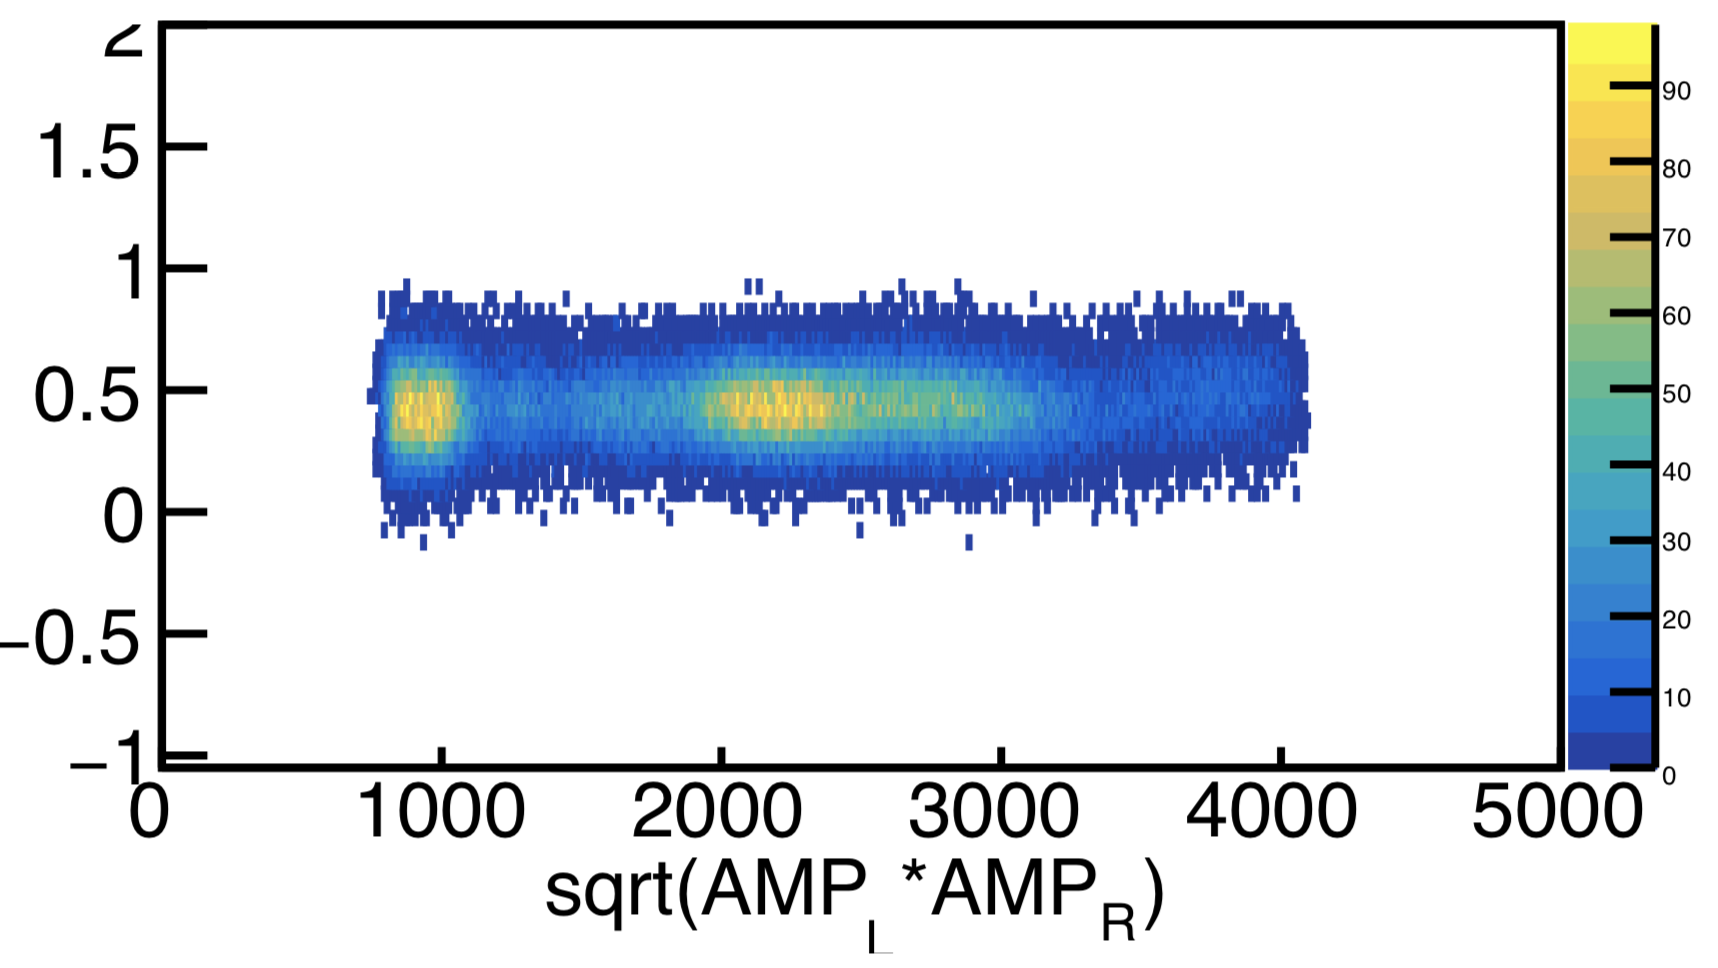
\includegraphics[width=0.8\textwidth]{bar_offset.png}
	\caption{Typcial time difference of bar mean time to a reference bar as a function of geometric mean of ADC pulse amplitude before corrections of relative bar offsets. The independence on amplitude shows a good time-walk calibration. The mean value of the y-axis gives the relativ time offset for this bar.}
	\label{fig:bar_off}
\end{figure*}

\subsection{BAND performance} 
%%% ----------------- Global offset subsection
\subsubsection{Global offset}
\label{sec:global_offset}
A final global time offset is required to align the BAND with production data. Due to low rates in the angular coverage of the BAND, 
high-statistics data files must be used. 
In Fig.~\ref{fig:final_offset} (left) the time of flight spectrum is shown for each bar applying all calibrations described in the previous section. The spectrum is zoomed to the area of the photon peak which is used to determine the final global time offset calibration. The two peaks are the two groups of long and short bars which have different length of fiber optic cable installed. Therefore, a global offset is determined for each group independently assuming the known time of flight for photons. Fig.~\ref{fig:final_offset} (right) displays the time difference between the expected photon arrival time and the measured time corrected for the global offsets for all bars. One can see that after the corrections all bars are well aligned in time.
\begin{figure*}[h!]
	\centering
		\includegraphics[width=0.48\textwidth]{global_single_bar_all_runs.pdf}
		\includegraphics[width=0.48\textwidth]{global_single_bar_result.pdf}
	\caption{Left: Time of flight spectrum over all each around the photon peak before the global offset correction. Time of flight spectrum over all bars relative to the expected photon ToF after  the global offset correction. All bars are aligned.}
	\label{fig:final_offset}
\end{figure*}

\subsubsection{Time of Flight resolution}
Fig.~\ref{fig:tof_resolution} shows the obtained ToF resolutions for each bar. The resolutions are obtained from a Gaussian fit of the difference of the mean time of a bar to a reference bar.
In addition, an minimum energy deposition cut has been applied to remove events which are not of interest in the physics analysis. One can see that all bars are below the design resolution of
300 \si{\pico\s}. 
\begin{figure*}[h!]
	\centering
		\includegraphics[width=0.48\textwidth]{tof_resolution.pdf}
	\caption{ToF resolution as a function for every bar. All bars are well below the required 300 \si{\pico\s}. {\color{red} Update Figure with an energy deposit cut to show actually the good time resolution}}
	\label{fig:tof_resolution}
\end{figure*}

{\color{red} The current picture is without a energy deposit cut hence giving worse time resolution. Update Figure with an energy deposit cut.}
%%% ----------------- Neutral veto subsection
%\subsubsection{Neutral veto algorithm}

%%% ----------------- Photon-neutron subsection
\subsubsection{Neutron identification}
{\color{red} it would be good to update this section to ToF/m selection instead of ToF}
The neutron identification for production data is done by cuts on time-of-flight. Fig.~\ref{fig:tof} shows such a spectrum of events from production data where an electron was measured in coincidence in CLAS12 in the reaction $ed \rightarrow e'nX$. In addition, a minimum energy deposition cut of 5 \si{\MeV/\clight} has been applied for BAND hits. One can clearly see two separated peaks for photons and neutrons over a flat background from accidentals. The neutron peak corresponds to momenta between $200$ and $600$ \si{\MeV/\clight}.
The neutron selection in the physics analysis is based on $\beta$ or ToF per pathlength (inverse $\beta$).

\begin{figure*}[h!]
	\centering
		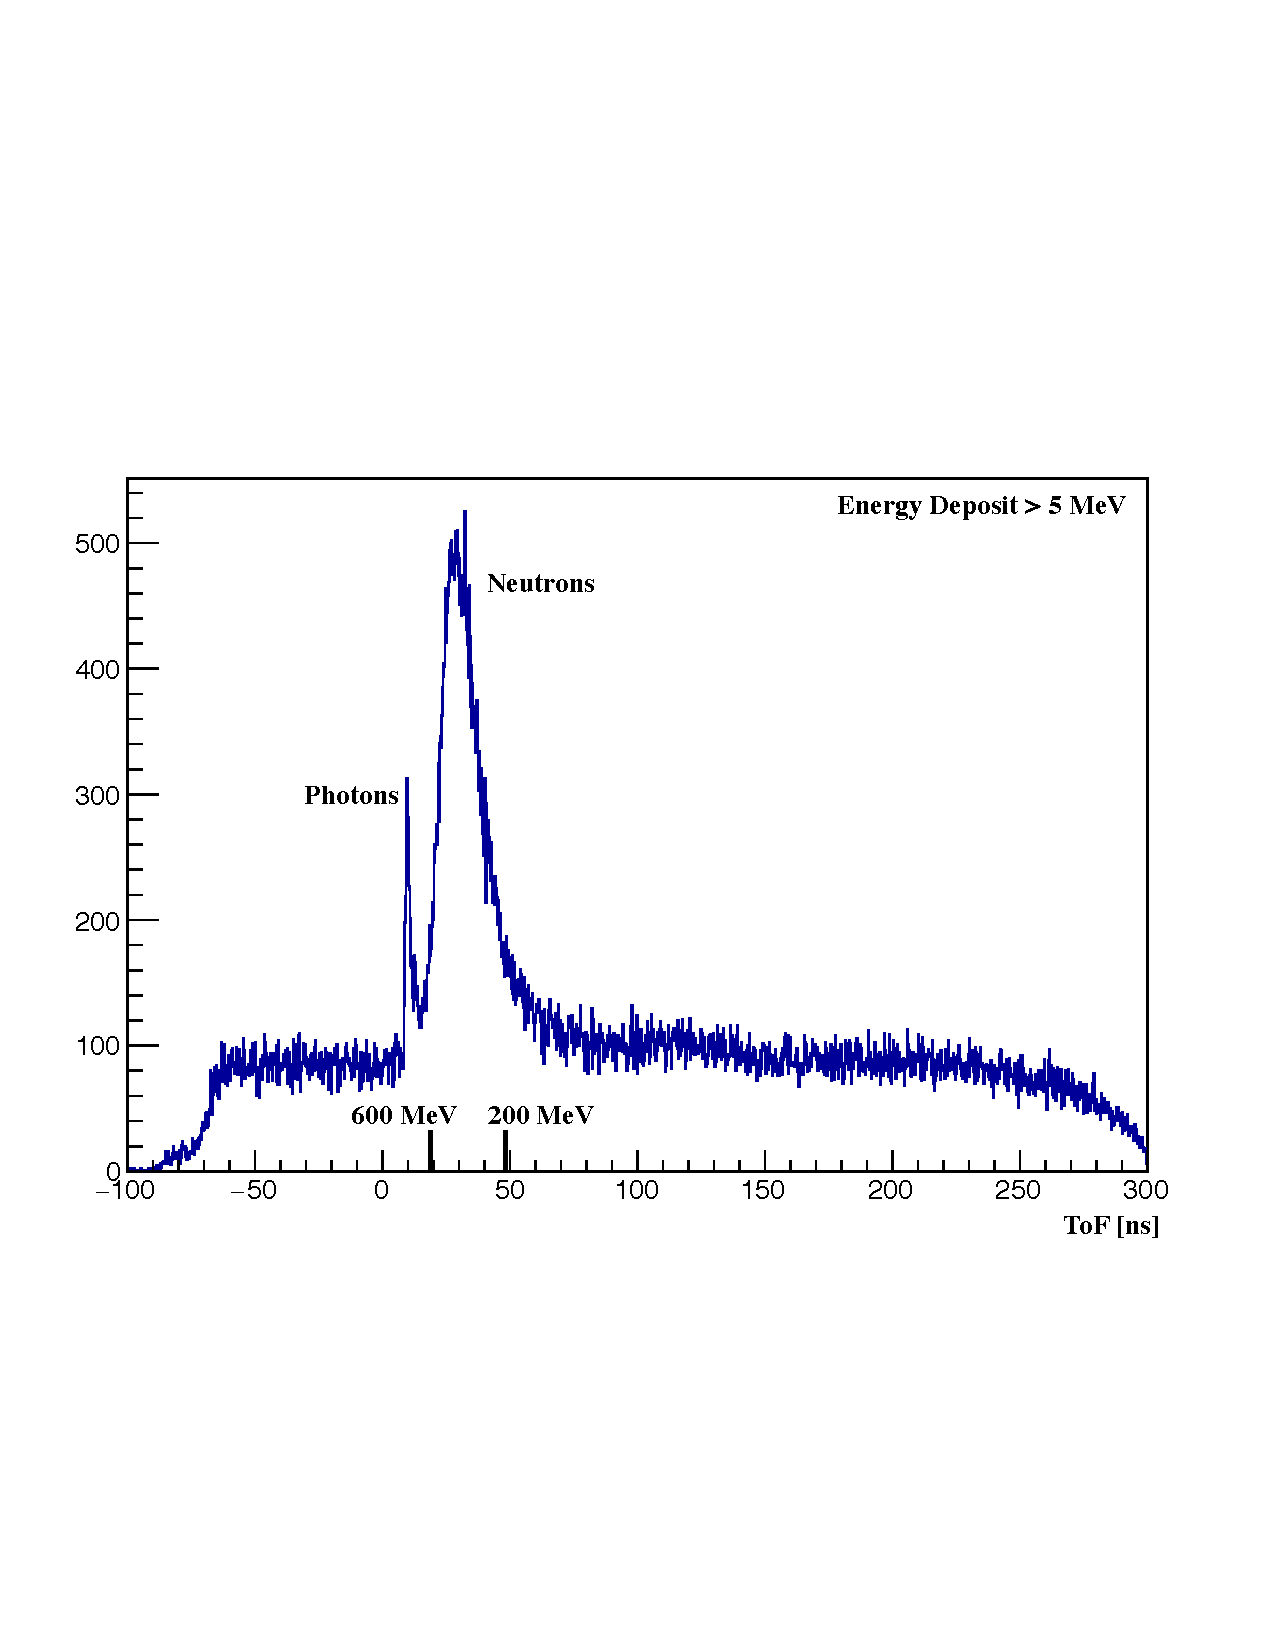
\includegraphics[width=0.96\textwidth]{tof-labels.pdf}
	\caption{Time-of-flight spectrum of BAND in coincidence with electrons measured in CLAS12 from production data. Clearly a photon and neutron peak is visible over a flat background from accidentals. The neutron peak corresponds to momenta  between $200$ and $600$ \si{\MeV/\clight}}
	\label{fig:tof}
\end{figure*}

%%% ----------------- Efficiency, resolution subsection
\subsubsection{Neutron efficiency}
TO DO: Efficiency results from GEANT simulation



%%%%%%%%%%%%%%%%%%%%%%%%%%%%%%%%%%%%%%%%%%%%%%%%%%%%%%%%%%%%%%%%%%%%%%%%%%%%%%%%%%%%%%%%%%%%%%%%%%%

\section{Summary}
The details and performance of the Backward Neutron Detector is presented in this paper. The detector is currently installed in front of the CLAS12 spectrometer at Jefferson Lab to measure neutrons with momenta between $0.25$ and $0.6$ \si{\GeV/\clight}.  It consists of scintillator bars with PMT readout on both ends.
After various calibrations a time of flight resolution of better than 300 \si{\pico\s} has been obtained for each scintillator bar consisted with design expectations from test measurements of components. A clear separation of backward going photons and neutrons reaching the detector can be seen in time of flight spectra for events where an electron is detected in CLAS12 of the reaction $e+d \rightarrow e'+X$, hence showing the excellent performance of the detector during the experiment.

The expected neutron efficiency from simulation is $35$\% . In the future, an analysis of data from exclusive $ed \rightarrow e'pn$ events collected at Jefferson Lab will allow to verify the expected efficiency.

%%%%%%%%%%%%%%%%%%%%%%%%%%%%%%%%%%%%%%%%%%%%%%%%%%%%%%%%%%%%%%%%%%%%%%%%%%%%%%%%%%%%%%%%%%%%%%%%%%%

\section{Acknowledgements}

%%%%%%%%%%%%%%%%%%%%%%%%%%%%%%%%%%%%%%%%%%%%%%%%%%%%%%%%%%%%%%%%%%%%%%%%%%%%%%%%%%%%%%%%%%%%%%%%%%%
\clearpage

\section{Appendix}
%\begin{tabular}{  m{3em} | m{3em} | m{5em} | m{3em} | m{3em} | m{3em} | m{8em} }
%		\hline
%			Sector & Layer & Component & Length (\si{\centi\meter}) & PMTs  & $\sigma$ (\si{\pico\second}) & Nominal distance from target (\si{\centi\meter}) \\
%		\hline
%		\hline
%1	&1	&1	&160	&R7724	&XXX	&XXX\\ 
%1	&1	&2	&160	&R7724	&XXX	&XXX\\ 
%1	&1	&3	&160	&R7724	&XXX	&XXX\\ 
%2	&1	&1	&200	&R7724	&XXX	&XXX\\ 
%2	&1	&2	&200	&R7724	&XXX	&XXX\\ 
%2	&1	&3	&200	&R7724	&XXX	&XXX\\ 
%2	&1	&4	&200	&R7724	&XXX	&XXX\\ 
%2	&1	&5	&200	&R7724	&XXX	&XXX\\ 
%2	&1	&6	&200	&R7724	&XXX	&XXX\\ 
%2	&1	&7	&200	&R7724	&XXX	&XXX\\ 
%3	&1	&1	&50	&ET9214	&XXX	&XXX\\ 
%3	&1	&2	&50	&ET9214	&XXX	&XXX\\ 
%3	&1	&3	&50	&ET9214	&XXX	&XXX\\ 
%3	&1	&4	&50	&ET9214	&XXX	&XXX\\ 
%3	&1	&5	&50	&ET9214	&XXX	&XXX\\ 
%3	&1	&6	&50	&ET9214	&XXX	&XXX\\ 
%4	&1	&1	&50	&ET9214	&XXX	&XXX\\ 
%4	&1	&2	&50	&ET9214	&XXX	&XXX\\ 
%4	&1	&3	&50	&ET9214	&XXX	&XXX\\ 
%4	&1	&4	&50	&ET9214	&XXX	&XXX\\ 
%4	&1	&5	&50	&ET9214	&XXX	&XXX\\ 
%4	&1	&6	&50	&ET9214	&XXX	&XXX\\ 
%1	&2	&1	&160	&R7724	&XXX	&XXX\\ 
%1	&2	&2	&160	&R7724	&XXX	&XXX\\ 
%1	&2	&3	&160	&R7724	&XXX	&XXX\\ 
%2	&2	&1	&200	&R7724	&XXX	&XXX\\ 
%2	&2	&2	&200	&R7724	&XXX	&XXX\\ 
%2	&2	&3	&200	&R7724	&XXX	&XXX\\ 
%2	&2	&4	&200	&R7724	&XXX	&XXX\\ 
%2	&2	&5	&200	&R7724	&XXX	&XXX\\ 
%2	&2	&6	&200	&R7724	&XXX	&XXX\\ 
%2	&2	&7	&200	&R7724	&XXX	&XXX\\ 
%3	&2	&1	&50	&ET9214	&XXX	&XXX\\ 
%3	&2	&2	&50	&ET9214	&XXX	&XXX\\ 
%3	&2	&3	&50	&ET9214	&XXX	&XXX\\ 
%3	&2	&4	&50	&ET9214	&XXX	&XXX\\ 
%3	&2	&5	&50	&ET9214	&XXX	&XXX\\ 
%3	&2	&6	&50	&ET9214	&XXX	&XXX\\ 
%4	&2	&1	&50	&ET9214	&XXX	&XXX\\ 
%4	&2	&2	&50	&ET9214	&XXX	&XXX\\ 
%4	&2	&3	&50	&ET9214	&XXX	&XXX\\ 
%4	&2	&4	&50	&ET9214	&XXX	&XXX\\ 
%4	&2	&5	&50	&ET9214	&XXX	&XXX\\ 
%4	&2	&6	&50	&ET9214	&XXX	&XXX\\ 
%1	&3	&1	&160	&R7724	&XXX	&XXX\\ 
%1	&3	&2	&160	&R7724	&XXX	&XXX\\ 
%1	&3	&3	&160	&R7724	&XXX	&XXX\\ 
%2	&3	&1	&200	&R7724	&XXX	&XXX\\ 
%2	&3	&2	&200	&R7724	&XXX	&XXX\\ 
%2	&3	&3	&200	&R7724	&XXX	&XXX\\ 
%2	&3	&4	&200	&R7724	&XXX	&XXX\\ 
%2	&3	&5	&200	&R7724	&XXX	&XXX\\ 
%2	&3	&6	&200	&R7724	&XXX	&XXX\\ 
%2	&3	&7	&200	&R7724	&XXX	&XXX\\ 
%3	&3	&1	&50	&ET9214	&XXX	&XXX\\ 
%3	&3	&2	&50	&ET9214	&XXX	&XXX\\ 
%3	&3	&3	&50	&ET9214	&XXX	&XXX\\ 
%3	&3	&4	&50	&ET9214	&XXX	&XXX\\ 
%3	&3	&5	&50	&ET9214	&XXX	&XXX\\ 
%3	&3	&6	&50	&ET9214	&XXX	&XXX\\ 
%4	&3	&1	&50	&ET9214	&XXX	&XXX\\ 
%4	&3	&2	&50	&ET9214	&XXX	&XXX\\ 
%4	&3	&3	&50	&ET9214	&XXX	&XXX\\ 
%4	&3	&4	&50	&ET9214	&XXX	&XXX\\ 
%4	&3	&5	&50	&ET9214	&XXX	&XXX\\ 
%4	&3	&6	&50	&ET9214	&XXX	&XXX\\ 
%1	&4	&1	&160	&R7724	&XXX	&XXX\\ 
%1	&4	&2	&160	&R7724	&XXX	&XXX\\ 
%1	&4	&3	&160	&R7724	&XXX	&XXX\\ 
%2	&4	&1	&200	&R7724	&XXX	&XXX\\ 
%2	&4	&2	&200	&R7724	&XXX	&XXX\\ 
%2	&4	&3	&200	&R7724	&XXX	&XXX\\ 
%2	&4	&4	&200	&R7724	&XXX	&XXX\\ 
%2	&4	&5	&200	&R7724	&XXX	&XXX\\ 
%2	&4	&6	&200	&R7724	&XXX	&XXX\\ 
%2	&4	&7	&200	&R7724	&XXX	&XXX\\ 
%3	&4	&1	&50	&ET9214	&XXX	&XXX\\ 
%3	&4	&2	&50	&ET9214	&XXX	&XXX\\ 
%3	&4	&3	&50	&ET9214	&XXX	&XXX\\ 
%3	&4	&4	&50	&ET9214	&XXX	&XXX\\ 
%3	&4	&5	&50	&ET9214	&XXX	&XXX\\ 
%3	&4	&6	&50	&ET9214	&XXX	&XXX\\ 
%4	&4	&1	&50	&ET9214	&XXX	&XXX\\ 
%4	&4	&2	&50	&ET9214	&XXX	&XXX\\ 
%4	&4	&3	&50	&ET9214	&XXX	&XXX\\ 
%4	&4	&4	&50	&ET9214	&XXX	&XXX\\ 
%4	&4	&5	&50	&ET9214	&XXX	&XXX\\ 
%4	&4	&6	&50	&ET9214	&XXX	&XXX\\ 
%		\hline
%	\end{tabular}




\section*{References}

% Create the reference section using BibTeX:
\bibliography{band_nim_bib}


\end{document}
